% Outras Opções:
%   * openright  -- Força início de capítulos em páginas ímpares (padrão da
%                   biblioteca)
%   * oneside    -- Desliga frente-e-verso
%   * nominatalocal -- Lê os dados da nominata do arquivo nominatalocal.def
\documentclass[ppgc,diss,english,openright]{iiufrgs}

\usepackage[utf8]{inputenc}
\usepackage[alf,abnt-emphasize=bf]{abntex2cite}	% pacote para usar citações abnt

\usepackage{lmodern}
\usepackage{amsmath}
\usepackage{amsthm}
\usepackage{enumitem}
\usepackage{listings}
\usepackage{xcolor}
\usepackage{amsfonts}
\usepackage{newtxtext,newtxmath}
\usepackage{semantic}
\usepackage{float}
\usepackage{mdframed}
\usepackage{stmaryrd}
\usepackage{multicol}
\usepackage{graphicx}
\usepackage[color=red]{todonotes}

\usepackage{times}
\usepackage{palatino}
\usepackage{mathptmx}
\usepackage[all,knot,arc,import,poly]{xy}

\theoremstyle{plain}
\newtheorem{thm}{Theorem}[chapter]

\theoremstyle{definition}
\newtheorem{mydef}[thm]{Definition}
\newtheorem{example}[thm]{Example}

\def\changemargin#1#2{\list{}{\rightmargin#2\leftmargin#1}\item[]}
\let\endchangemargin=\endlist

\newenvironment{intuition}{\begin{changemargin}{1cm}{1cm}}{\end{changemargin}}

\newcommand{\diagram}[1]{\centerline{\xymatrix{#1}}}
\newcommand{\grule}{$p = (L \leftarrow K \rightarrow R) $}
\newcommand{\rulesequence}{$p_0,\ldots,p_{n-1},p_n$}

% avoid LaTeX Font Warning: Font shape `U/stmry/b/n' undefined
\SetSymbolFont{stmry}{bold}{U}{stmry}{m}{n}

\title{Attributes in Graph Transformation Systems using the Double Pushout Approach}
\author{Santos Bezerra}{Jonas}
\advisor[Prof$^a$.]{Ribeiro}{Leila}
%\date{maio}{2001}
\location{Porto Alegre}{RS}

% itens individuais da nominata podem ser redefinidos com os comandos
% abaixo:
% \renewcommand{\nominataReit}{Prof\textsuperscript{a}.~Wrana Maria Panizzi}
% \renewcommand{\nominataReitname}{Reitora}
% \renewcommand{\nominataPRE}{Prof.~Jos{\'e} Carlos Ferraz Hennemann}
% \renewcommand{\nominataPREname}{Pr{\'o}-Reitor de Ensino}
% \renewcommand{\nominataPRAPG}{Prof\textsuperscript{a}.~Joc{\'e}lia Grazia}
% \renewcommand{\nominataPRAPGname}{Pr{\'o}-Reitora Adjunta de P{\'o}s-Gradua{\c{c}}{\~a}o}
% \renewcommand{\nominataDir}{Prof.~Philippe Olivier Alexandre Navaux}
% \renewcommand{\nominataDirname}{Diretor do Instituto de Inform{\'a}tica}
% \renewcommand{\nominataCoord}{Prof.~Carlos Alberto Heuser}
% \renewcommand{\nominataCoordname}{Coordenador do PPGC}
% \renewcommand{\nominataBibchefe}{Beatriz Regina Bastos Haro}
% \renewcommand{\nominataBibchefename}{Bibliotec{\'a}ria-chefe do Instituto de Inform{\'a}tica}
% \renewcommand{\nominataChefeINA}{Prof.~Jos{\'e} Valdeni de Lima}
% \renewcommand{\nominataChefeINAname}{Chefe do \deptINA}
% \renewcommand{\nominataChefeINT}{Prof.~Leila Ribeiro}
% \renewcommand{\nominataChefeINTname}{Chefe do \deptINT}

\keyword{Graph Transformations}
\keyword{Use Cases}

\newcommand{\pu}{processing unit}
\newcommand{\Pu}{Processing unit}
\newcommand{\pus}{processing units}
\newcommand{\Pus}{Processing units}
\newcommand{\envid}{env_{id}}

\definecolor{kwcolor}{rgb}{0,0.5,0}
\definecolor{bgcolor}{rgb}{0.98, 0.98, 0.98}
\definecolor{numbercolor}{rgb}{0.1,0.1,0.1}

\lstset{
  keywordstyle=\bfseries\underbar,
  stringstyle=\itshape,
  basicstyle=\small\ttfamily,
  frame=bt,
  framerule=1pt,
  numbers=left,
  numbersep=10pt,
  numberstyle=\scriptsize\color{numbercolor},
  backgroundcolor=\color{bgcolor},
  tabsize=2
}

\lstdefinelanguage{l1}
{keywords={let, letrec, in, if, then, else, end, unused}%
  sensitive=true,
  alsoletter={\$},
  comment=[l]{\#},
  string=[b]"
}

\lstdefinelanguage{acqua-ir}
{keywords={unused, EnvNew, EnvAdd, Call, unused}%
  sensitive=true,
  alsoletter={\$},
  comment=[l]{\#},
  string=[b]"
}

\graphicspath{ {images/} }
%\captionsetup[table]{skip=10pt}
\newmdenv[leftline=false,rightline=false]{openframe}




\sloppy
\begin{document}

  \maketitle
  \clearpage

  % dedicatoria
  \clearpage
  \begin{flushright}
    \mbox{}\vfill
    {\sffamily\itshape
    ``Poste, kiam \^si pripensis la aferon,\\
    \^si opiniis ke tio ja estis mirinda,\\
    sed kiam \^gi okazis \^cio \^sajnis tute natura.''\\}
    --- \textsc{Alico en Mirlando}
  \end{flushright}

  % agradecimentos
  \chapter*{Agradecimentos}
  Yet to come\ldots
  
  \begin{abstract}
    about:verigraph
  \end{abstract}

  \begin{listofabbrv}{SPMD}
          \item[DPO] Double Pushout
          \item[GTS] Graph Transformation System
          \item[NAC] Negative Application Condition
          \item[PB] Pullback
          \item[PO] Pushout
  \end{listofabbrv}

  \begin{listofsymbols}{$\alpha\beta\pi\omega$}
         \item[$\leftarrow$] Morphism
  \end{listofsymbols}

  \listoffigures
  \tableofcontents

  \chapter{Introduction}

Graph grammars are a suitable formalism to model complex systems in an intuitive and precise manner, providing both a graphical language and a solid formal background for systems analysis. In this framework, system states are modelled as graphs, while transitions between different states are modelled as graph transformation rules~\cite{Ehrig2006}. A graph transformation rule generically has the form $L \xRightarrow{p} R$, where there is at least one left side graph $L$ containing a pattern to be found (a match) in order for the rule to be applied over an instance graph and a right side graph $R$ corresponding to the effect of applying such a rule. Moreover, there are also additional structures that may be used as complements of rules to better tune which kinds of matches are acceptable to perform a transformation, for instance: Graph Constraints, Negative Application Conditions (NACs) and Nested Application Conditions, to cite some of the most commonly used.

There exist several approaches that might not only change the exact format of a rule, but also define different ways a rule can be applied over a given match. Only considering the domain of Category Theory there is already a handful of different approaches to graph grammars: the Single Pushout (SPO), Double Pushout (DPO), Sesqui-Pushout (SqPO), AGREE, among others. Each approach has its own advantages/disadvantages regarding the kinds of  ``operations'' they allow or forbid in the system under modelling. 
In spite of that, whichever approach is used, they all provide a way to describe the behaviour of the system together with means to analyse several properties about this behaviour, such as termination, concurrency and reachable states. Among the several analysis techniques provided by graph grammars, we have:

\begin{itemize}
  \item Critical Pair Analysis and Critical Sequence Analysis: critical pair analysis allows us to verify which rules conflict with (i.e. prohibit) the application of another and why; critical sequence analysis, which rules depend on the execution of others to be applied and why~\cite{Lambers2008a}; such analyses provide insights about the possible execution flows of the system.
  \item Calculation of Concurrent Rules: a concurrent rule summarizes in one rule the combined results of applying several different rules. In other words, it represents the combination of several different rules which can be then applied as a ``one step'' transformation rule~\cite{Lambers2008,BezerraETMF2016}.
  \item State Space Exploration and Model Checking: permits to verify, in an exhaustive fashion, whether the (graph grammar) model of a system satisfies a given specification and to prove the satisfaction of its properties~\cite{Rensink2004}.
  \item Unfolding, Graph Processes, Occurrence Graph Grammars and Canonical Derivations: they are all different means to provide the semantics of Graph Grammars, allowing us to check which graphs belong to the language of a grammar and/or which concrete derivations are possible within that grammar~\cite{Corradini1996,Ribeiro1996}.
\end{itemize}

Graph grammars have found a wide range of applications within Computer Science, specially in the field of model-driven software development, where the transformation of visual models is a vital part of the process, therefore a natural application of graph grammars~\cite{Rozenberg1997}.
As evidence of such suitability, several non-trivial systems have been modelled and studied under the optics of graph grammars, such as telephone communications~\cite{Ribeiro1996}, elevator control~\cite{Lambers2010}, railroad control~\cite{Pennemann2009} and integration of service-oriented systems~\cite{Giese2015}.
Furthermore, there are a number of software tools to support the use of graph grammars, such as AGG, a tool environment for algebraic graph transformation~\cite{Taentzer2000}; Groove, a tool for state space generation~\cite{Rensink2004} and Verigraph, a software specification and verification tool based on graph rewriting~\cite{verigraph}.

Besides its powerful applications, the use of graph grammars as a framework for modelling systems provides us with a great advantage over other formalisms: it makes it possible for non-specialists in the field to generate graph grammar models of a system and then benefit from the rigorous analyses it offers without the need for a deep understanding of its underlying theory. For example, ~\cite{Junior2015,BezerraWEIT2016,Cota2017} explain how to generate graph grammars from a set of textual requirement documents such as use cases, functional specifications and other kinds of guidelines by means of a systematic methodology. They also present guidance towards using different graph grammars analysis techniques in order to improve and verify these documents and, consequently, the systems they describe.

The field of Graph Grammars is a very active one, and researches continuously develop new ideas, such as new graph transformation approaches (e.g. Sesqui-Pushout, AGREE), analysis techniques (e.g. Essential Critical Pairs), tools (e.g. Verigraph) and ways to apply them.
Additionally, we may also benefit from the combination of already existing techniques, which is what we do in this thesis.
In our work, we combine two concepts of the Graph Grammar Theory: Occurrence Graph Grammars, defined for the SPO and DPO approaches by~\cite{Ribeiro1996, Corradini1996}, with Negative Application Conditions, defined generically by~\cite{Habel1996}, which has not been done so far.

Occurrence Graph Grammars provides a semantics for Graph Grammars encoded in structures that are also Graph Grammars themselves. 
This semantics, which tells us which graphs are part of the grammar language and which graph transformations are possible within the context of the original grammar, may be used for the analysis of the system execution in a summarized fashion and also be used for practical applications, such as test cases generation, without the necessity to use a supplementary structure or formalism.

Negative Application Conditions (NACs) are extensions of rules encoding patterns that, if found in the match of a rule, forbids the transformation. In theory, they do not give any more expressive power to a graph grammar than using only rules without them~\cite{Habel1996}. In practice, they allow the modelling of systems in a much more concise and compact manner. Therefore they became really necessary in the modelling of complex, real-like systems~\cite{Corradini2013, Corradini2014}.

Our work here consists of the development of an extension for the framework of Occurrence Graph Grammars in the Double Pushout (DPO) approach in order to incorporate Negative Application Conditions, alongside with the implementation of this extension in the Verigraph system, a generic graph rewriting system based on Category Theory and written in Haskell. This implementation choice makes possible for the source code of the tool to be close to the theory domain as well as allowing other researches to implement new approaches or different models of graphs while benefiting from the already implemented techniques (as long as they conform to the categorial constructions).

%We believe that the use of graph grammars as a model for the generation of test cases and oracles may improve the reliability of the testing activity by using the solid formal semantics of the formalism, while requiring little theoretical expertise from the user. The main objective of this thesis can be summarized as follows:

%\begin{intuition}
%  \center{\textit{Given the graph grammar model of a software system, how can a set of relevant test cases and oracles be generated for the system?}}
%\end{intuition}\hfill\break

Thus, the main contributions of this thesis can be summarized as (1) the creation of an extension  to the framework of Occurrence Graph Grammars (in the DPO approach) in order to include Negative Application Conditions and (2) the implementation of this extension in Verigraph, a software specification and verification system based on graph transformations, which is now also the first tool in the field to implement the construction of Occurrence Graph Grammars for general Graph Grammars, even when considering OGGs without NACs.

\hfill \break
\textbf{Structure of the Thesis:}

\begin{description}
	\item[Chapter~\ref{ch:gts}:] In this chapter we review the basic notions of graph transformation systems, specifically under the Double-Pushout (DPO) approach. We also introduce Negative Application Conditions (NACs) and the basic notions of parallel and sequential independence of rules, which are needed for the construction of Occurrence Graph Grammars with NACs.

  \item[Chapter~\ref{ch:process}:] In this chapter we first present an overview of doubly-typed graph grammars and other concepts necessary to accomplish the construction of Occurrence Graph Grammars, as well as how these Occurrence Grammars can be used to represent the semantics of their original grammar. After reviewing these concepts, we present our extension to previous works in Occurrence Graph Grammars to include the notion of Negative Application Conditions, which is part of our thesis contribution.

  \item[Chapter~\ref{ch:verigraph}:] This chapter presents an overview of the Verigraph system, which was used to implement the techniques presented in this thesis. Verigraph in itself represents a novelty in the field of graph transformations, being the first tool in the area implemented in a functional language, which favoured its source code to be very close to the problem domain itself.

  \item[Chapter~\ref{ch:tests}:] This chapter explains in depth the step-by-step construction of an Occurrence Graph Grammar with the help of some running examples. Additionally, it demonstrates how this was implemented in Verigraph, while also providing some insight about how it can be used for test cases generation.

  \item[Chapter~\ref{ch:related-work}:] This chapter discuss related work to the one presented in this thesis. Specifically focusing on the literature about the Semantics of Graph Grammars and how to use it for test cases generation. It also lists some software tools related to Verigraph.

  \item[Chapter~\ref{ch:conclusions}:] This chapter summarizes our results and presents our conclusions. Moreover, it shows remaining open problems and future work.

  \item[Appendix~\ref{app:category-theory}:] This appendix contains a brief review of category theory and the categorial constructions used in this thesis.

  %\item[Appendix~\ref{app:use-cases}] This appendix contains the use cases and the modelled graph grammar used as a case study on section~\ref{ch:tests}.
\end{description}

  \chapter{Category Theory and Graph Grammars}\label{ch:gts}

\section{Category Theory}

Category theory is a powerful mathematical framework, defined by~\cite{Eilenberg1945}, that provides an abstract way to reason about mathematical structures and the relationships between them.

Categories are particularly useful in Computer Science, having several applications such as design of programming languages, implementation techniques, semantic models, concurrency models, type theory, among others~\cite{Pierce1991}.

Category theory is also the basis for graph transformation systems, which is central to the work proposed in this thesis. Therefore, we present a brief introduction of the field and basic categorial constructions that will be necessary in this work.

\begin{definition}[Category]\label{def:category} A category \cat{C} consists of a collection of \emph{objects} and a collection of \emph{arrows} between objects (also called \emph{morphisms}) such that:

  \begin{enumerate}
    \item for all arrows $f : A \rightarrow B$, $g : B \rightarrow C$ and
$h : C \rightarrow D$, with objects $A,B,C,D$ not necessarily distinct, the composition of arrows is associative:

  $h \circ (g \circ f) = (h \circ g) \circ f$;
    \item for every object $A$ there is an \emph{identity} arrow $id_A : A \rightarrow A$ such that for any arrow $f : A \rightarrow B$:

  $id_B \circ f = f$ and $f \circ id_A = f$.
  \end{enumerate}

\end{definition}

\begin{example}[Category of Sets] \cat{Set} is the category whose objects are \emph{sets} and the arrows and the arrows are \emph{total functions} between sets. The proof follows form the fact that:

\begin{enumerate}
  \item given any sets $A,B,C,D$, for all total functions $f : A \rightarrow B$, $g : B \rightarrow C$ and $h : C \rightarrow D$ we have that $h \circ (g \circ f) = (h \circ g) \circ f$;

  \item given any sets $A$ and $B$, there exist \emph{identity} functions $id_A : A \rightarrow A$ such that for any function $f : A \rightarrow B$ such that $id_B \circ f = f$ and $f \circ id_A = f$.
\end{enumerate}
\end{example}

%\begin{example}[Category of Graphs] \cat{Graph} is the category whose objects are graphs and the arrows are \emph{total graph homomorphisms}, i.e. graphs morphisms that preserve sources and targets of edges (see Definitions~\ref{def:graph} and~\ref{def:graph-morphism}). \tinytodo{Put proof or remove it.}
%\end{example}

\begin{definition}[Diagram] Given a category \cat{C}, a diagram in \cat{C} is a collection of vertices and directed edges such that, if an edge in the diagram is named with an arrow $f$ and $f$ has domain $A$ and codomain $B$, then the outgoing vertex of the edge must be named $A$ and the incoming vertex $B$.

  A diagram is said to \emph{commute} if, for every pair of objects $A,B$, all the paths in the diagram from $A$ to $B$ are equal. In other words, each path in the diagram determines an arrow and these arrows are equal in \cat{C}. If the following diagram commutes than we can say that \mbox{$g' \circ f = f' \circ g$}.

\diagram{
  A\ar[r]^{f}\ar[d]_{g} & Y\ar[d]^{g'}\\
  X\ar[r]_{f'} & B
}

\end{definition}

\begin{definition}[Monomorphism, Epimorphism and Isomorphism] An arrow \mbox{$f : B \rightarrow C$} in a category \cat{C} is said to be a \emph{monomorphism} if, for any pair of arrows $g : A \rightarrow B$ and $h : A \rightarrow B$, we have that $f \circ g = f \circ h \Rightarrow g = h$.

\diagram{
  A\ar@<.5ex>[r]^{g}\ar@<-.5ex>[r]_{h} & B\ar[r]^{f} & C
}

  An arrow \morph{f}{A}{B} is said to be an \emph{epimorphism} if, for any pair of arrows \morph{g}{B}{C}, \morph{h}{B}{C}, we have that \mbox{$g \circ f = h \circ f \Rightarrow g = h$}.

\diagram{
  A\ar[r]^{f} & B\ar@<.5ex>[r]^{g}\ar@<-.5ex>[r]_{h} & C
}

  An arrow \morph{f}{A}{B} is an \emph{isomorphism} if there is an arrow \morph{f^{-1}}{B}{A}, the \emph{inverse} of $f$, such that \mbox{$f^{-1} \circ f = id_A$} and \mbox{$f \circ f^{-1} = id_B$}


\diagram{ 
  A\ar@<.5ex>[r]^{f} & B\ar@<.5ex>[l]^{f^{-1}}
}
\end{definition}

\iffalse
\begin{example}[Monomorphism, Epimorphism and Isomorphism Examples]

  In \cat{Set}, the monomorphism, epimorphism and isomorphism concepts correspond to injective, surjective and bijective functions, respectively.\tinytodo{put examples}

  \tinytodo{explain ``up to isomorphism''}

\end{example}
\fi

\subsection{Categorial Constructions}

Here we present basic categorial constructions that are used throughout in this work. Notice that this is not an extensive list, we present only the constructions necessary to our scope. For a more in-depth explanation of Category Theory and its application in Computer Science refer to~\cite{Pierce1991}.

\begin{definition}[Coproduct] Given two objects $A$ and $B$, their \emph{coproduct} (also called \emph{categorical sum}) is an object $A+B$ and two injection arrows \morph{i_A}{A}{A+B} and \morph{i_B}{B}{A+B} such that, for any other object $X$ and pair of arrows \morph{f}{A}{X} and \morph{g}{B}{X}, there is one unique arrow \morph{!}{A+B}{X} such that the following diagram commutes:

\diagram{
  A\ar[r]^{i_A}\ar[dr]_{f} & A+B\ar@{.>}[d]^{!} & B\ar[l]_{i_B}\ar[dl]^{g}\\
    & X   &
}

\end{definition}

\begin{example}[Coproducts in \cat{Set}] Coproducts can be used to generalize the notion of disjoint union. Figure~\ref{fig:gts:coproduct} shows an example of it in the category \cat{Set}\footnote{The morphisms are represented in an expanded notation to explicitly show how the mappings were done.}.

  Having the sets $A = \{1,2,3\}$ and $B = \{1,2\}$ as objects, we have that the set $A+B$ together with morphisms $i_A$ and $i_B$ is their coproduct: all elements of $A$ and $B$ are mapped to $A+B$, no elements from the source objects are identified in the target, and it is possible to find a unique function from $A+B$ to any other candidate satisfying the commutative restriction.

\begin{figure}[!ht]
  \centering
  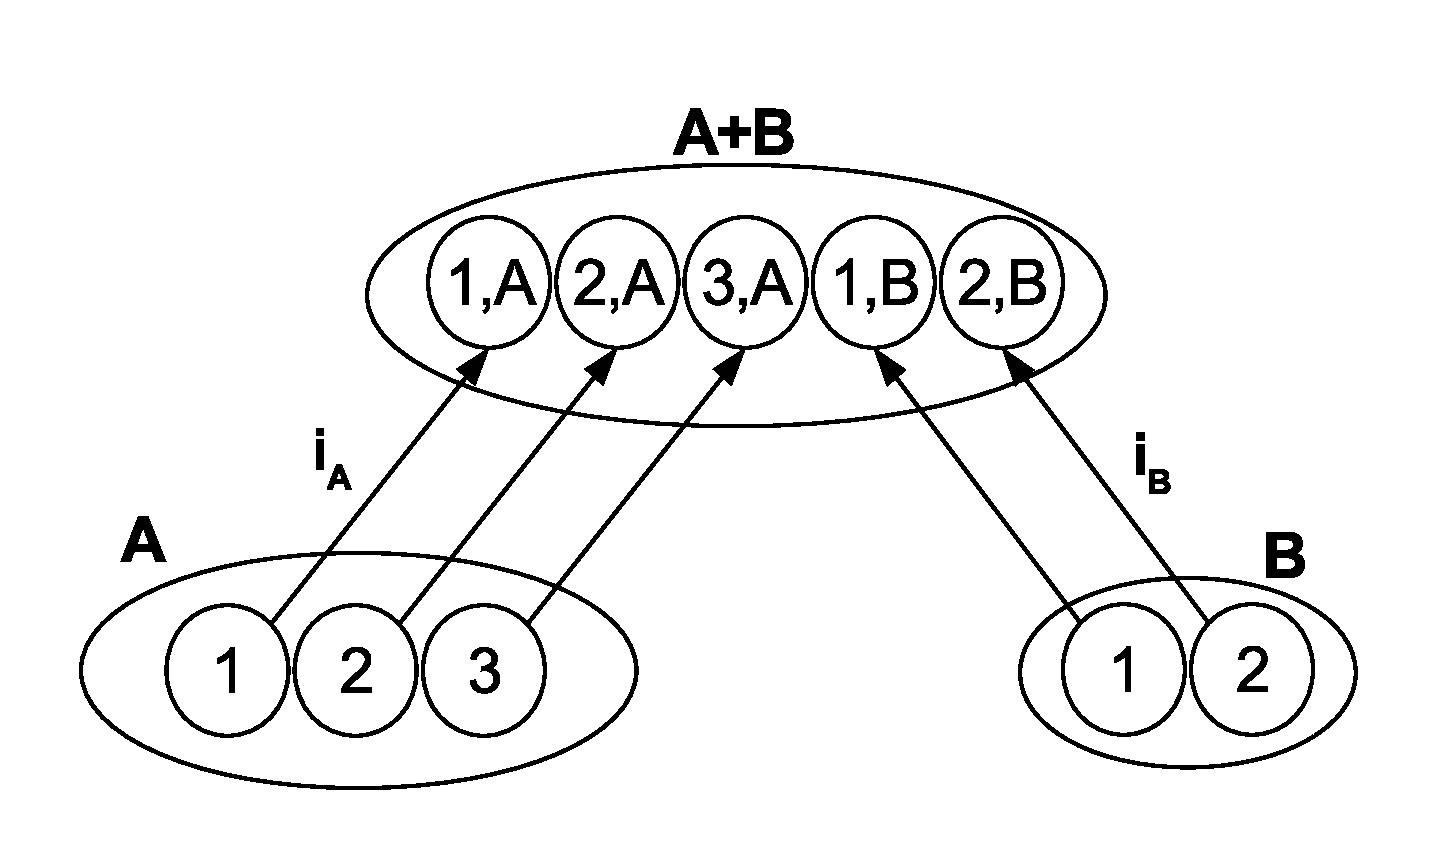
\includegraphics[scale=0.4]{images/gts/coproduct-open}
  \caption{A coproduct in \cat{Set}}\label{fig:gts:coproduct}
\end{figure}


  Take as a candidate a set $C = {(0,A),(1,A),(2,A),(3,A),(1,B},(2,B),(3,B)$. $C$ can not be a coproduct because we can not find a \emph{unique} arrow from $C$ to an arbitrary candidate $X$, as there are multiple choices due to the different possible functions mapping $A$ and $B$ to $C$. Also, an object such as $D = \{(1,A),(2,AB),(3,A),(1,B)\}$ can not be a coproduct because it is not possible to find an arrow from $D$ an $X$ such that the diagram commutes, because all the possible functions from $A$ and $B$ would identify some elements of the sources.

  Notice that $(A+B)' = \{(1,0),(2,0),(3,0),(1,1),(2,1)\}$ or $(A+B)'' = \{a,b,c,d,e\}$ or any other set with five elements would be equally valid as coproducts for this case. This is due to the fact the categories deal with their objects up to isomorphism, i.e. all this objects have the same format regardless of their internal representations.
\end{example}


\begin{definition}[Coequalizer] Given two objects $A$ and $B$ with two parallel morphisms \morph{f}{A}{B} \morph{g}{A}{B}, the coequalizer of the diagram is an object $X$ together with a morphism \morph{h}{B}{X} such that \mbox{$h \circ f = h \circ g$} and, for any other such objects $X'$ with a morphism $h'$, there is a unique morphism \morph{!}{X}{X'} such that the following diagram commutes.

\diagram{
  A\ar@<.5ex>[r]^{f}\ar@<-.5ex>[r]_{g} & B\ar[r]^{h}\ar[dr]_{h'} & X\ar@{.>}[d]^{!}\\
    &   & X'
}
\end{definition}

\begin{example}[Coequalizers in \cat{Set}] Coequalizers generalize the notion of smallest equivalence relation. Figure~\ref{fig:gts:coequalizer} shows the coequalizer for two functions from $A$ to $B$, let $f$ be the one represented with a solid line and $g$ the one with a dashed line.

\begin{figure}[!ht]
  \centering
  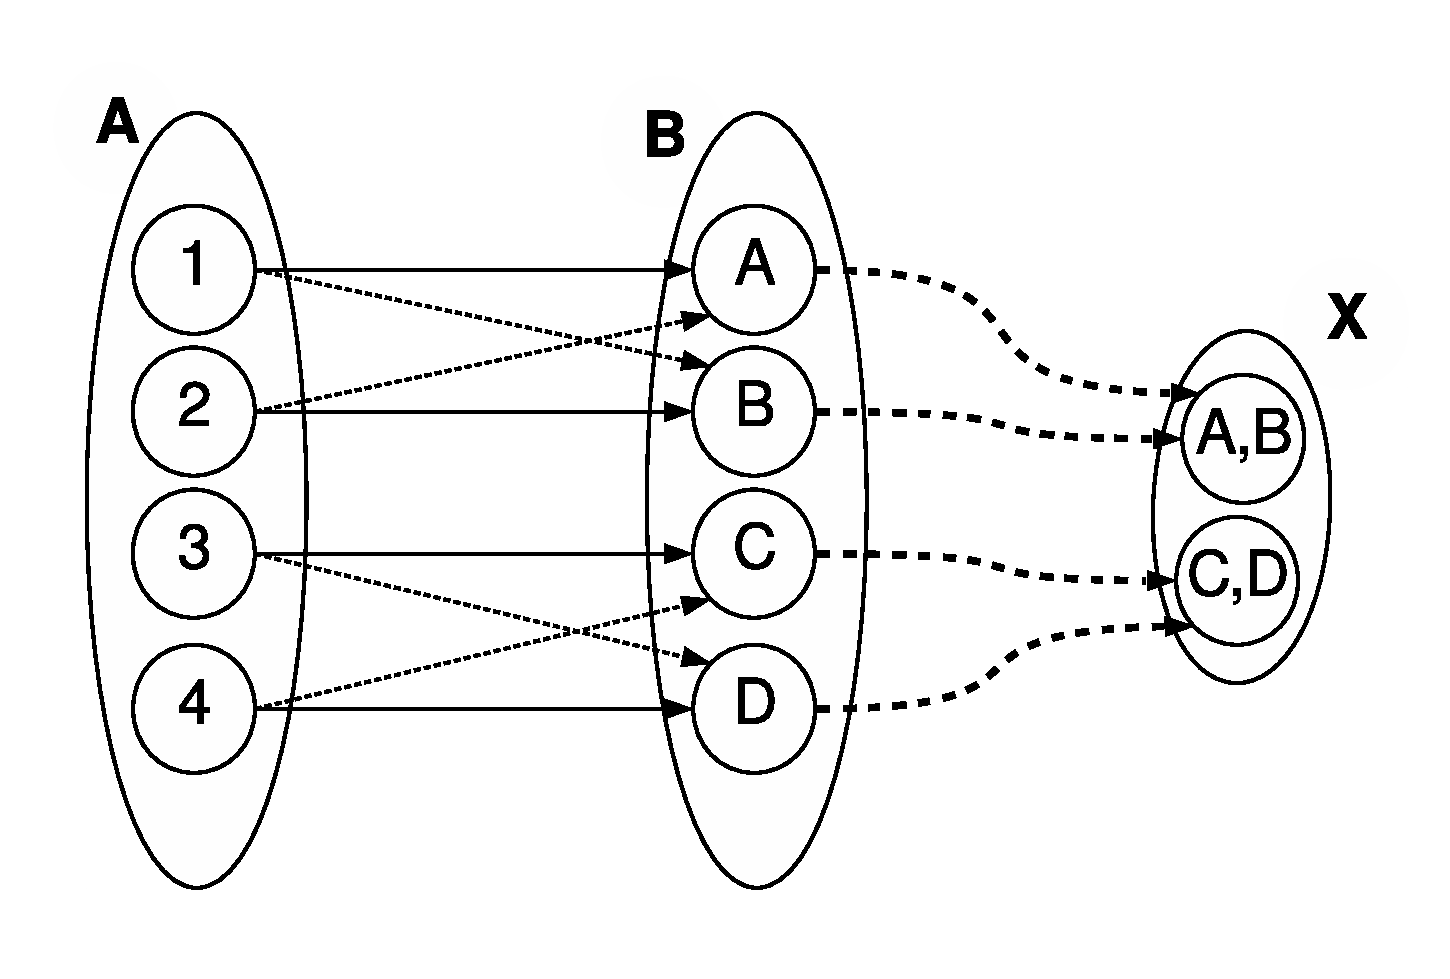
\includegraphics[scale=0.4]{images/gts/coequalizer}
  \caption{A coequalizer in \cat{Set}}\label{fig:gts:coequalizer}
\end{figure}

  It is easy to see that the the function $h$ from $B$ to $X$ corresponds to the equivalence relation that glues together the items that are identified by the functions $f$ and $g$. Notice that $X$ does not contain any other element which is not mapped from $B$ and no element in $X$ was glued together without respecting $f$ and $g$.

\end{example}

\begin{definition}[Pushout] Given a span of arrows \mbox{$B \xleftarrow{f} A \xrightarrow{g} C$}, its \emph{pushout} is an object $X$ together with a pair of arrows \morph{f'}{C}{X} and \morph{g'}{B}{X} such that (1) \mbox{$f' \circ g = g' \circ f$} and (2) for any other object $X'$ with morphisms \morph{i}{B}{X'} and \morph{j}{C}{X'} such that $i \circ f = j \circ g$ there is a unique morphism \morph{!}{X}{X'} such that \mbox{$i =$ $! \circ g'$} and \mbox{$j =$ $! \circ f'$}.

\diagram{
  A\ar[r]^{f}\ar[d]_{g} & B\ar[d]^{g'}\ar@/^1.1pc/[rdd]^{i} &\\
  C\ar[r]_{f'}\ar@/_1.1pc/[drr]_{j}       & X\ar@{.>}[dr]^{!}&\\
                &         &X'
}

\end{definition}

\begin{example}[Pushouts in \cat{Set}] A pushout in \cat{Set} can be seen on Figure~\ref{fig:gts:pushout}. Notice that a pushout maps all elements of sets $B$ and $C$ into set $X$, ``gluing'' the ones that are identified via the morphisms \morph{f}{A}{B} and \morph{g}{A}{C}.

\begin{figure}[!ht]
  \centering
  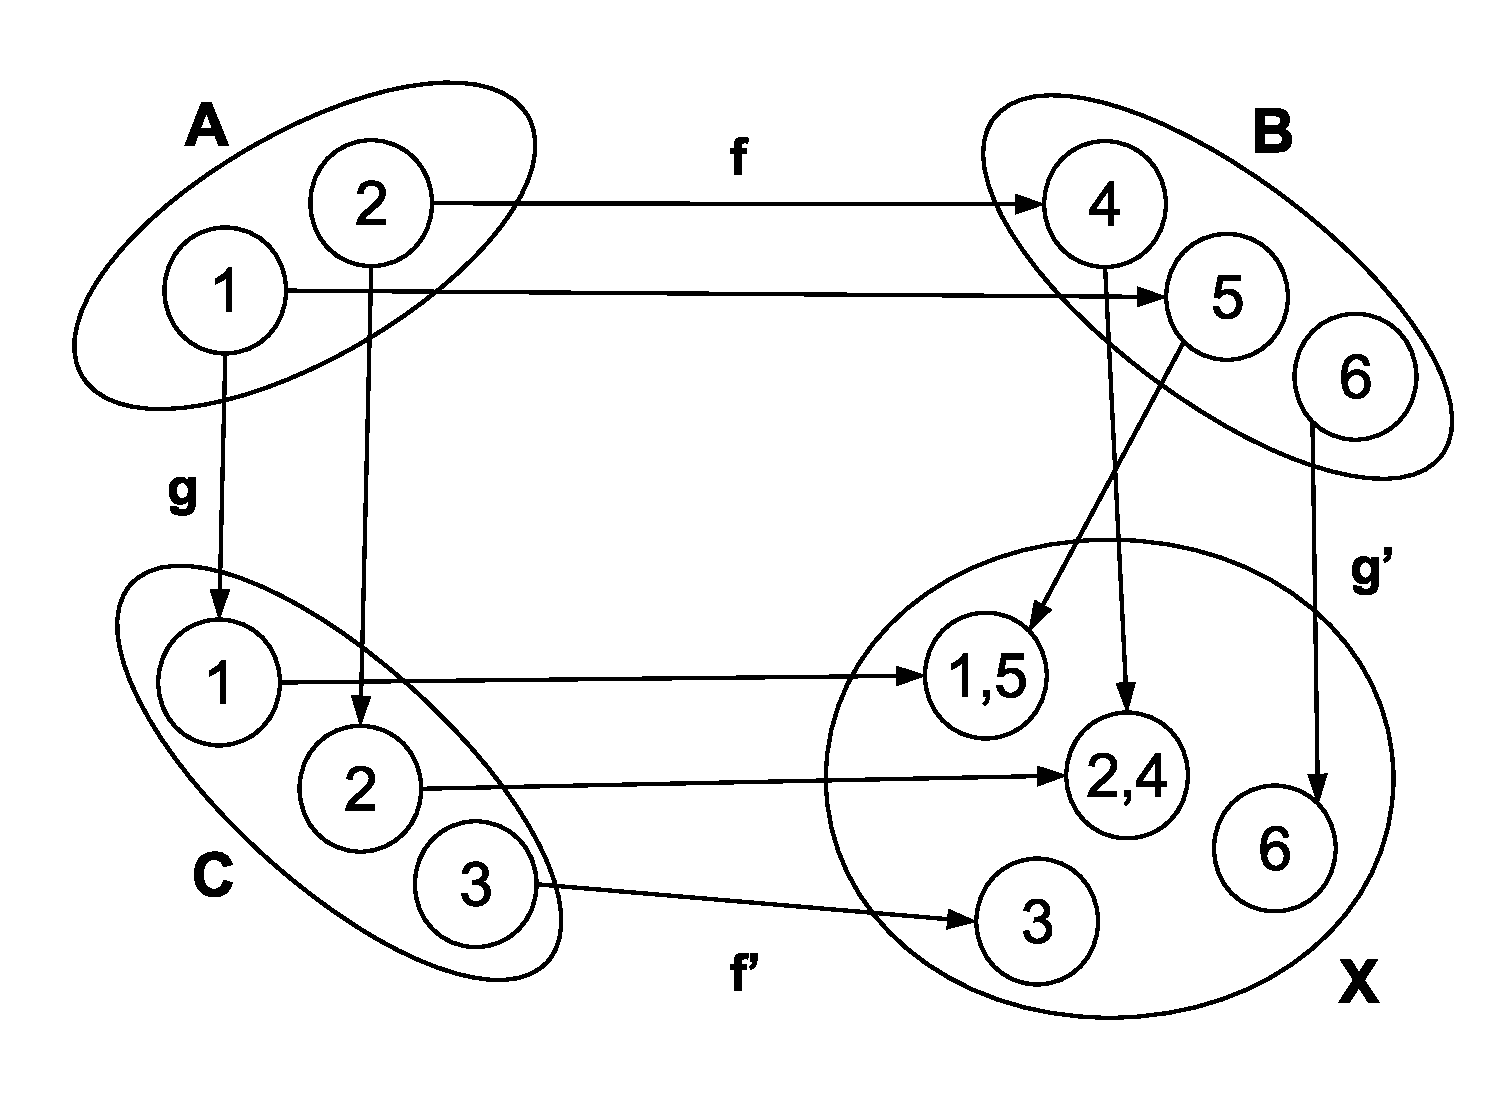
\includegraphics[scale=0.4]{images/gts/pushout}
  \caption{A pushout in \cat{Set}}\label{fig:gts:pushout}
\end{figure}

\end{example}

\begin{definition}[Colimit] Given a diagram $D$ in a category \cat{C}, a \emph{cocone} for $D$ is an object $X$ and a family of morphisms \morph{f_i}{D_i}{X} (one for each object $D_i$ in $D$), such that for each morphism $g$ in $D$ the outer part of the following diagram commutes.

\diagram{
  D_i\ar[rr]^{g}\ar[dr]_{f_i} &   & D_j\ar[dl]^{f_j}\\
      & X &   \\
}
\hfill

  A \emph{colimit} for a diagram $D$ is a cocone \{\morph{f_i}{D_i}{X}\} such that for any other cocone \{\morph{f'_i}{D'_i}{X'}\} there exists a unique morphism \morph{!}{X}{X'} such that the following diagram commutes for every $D_i$ in $D$.


\diagram{
  D_i\ar@/_1.1pc/[ddr]_{f'_i}\ar[rr]^{g}\ar[dr]_{f_i} &   & D_j\ar@/^1.1pc/[ddl]^{f'_j}\ar[dl]^{f_j}\\
      & X\ar@{.>}[d]^{!} &   \\
      & X'&    \\
}
\end{definition}

\begin{example}[Colimits in \cat{Set}] Colimits generalize several constructions such as disjoint unions, direct sums, coproducts, pushouts and others, where different objects of a diagram are ``glued'' together in one single object respecting commutativity.

  All previous examples of coproduct, coequalizer and pushout are special cases of colimits. Figure~\ref{fig:gts:colimit} shows a colimit for a diagram that can not be calculated in (one step) by any of the previous constructions.

\begin{figure}[!ht]
  \centering
  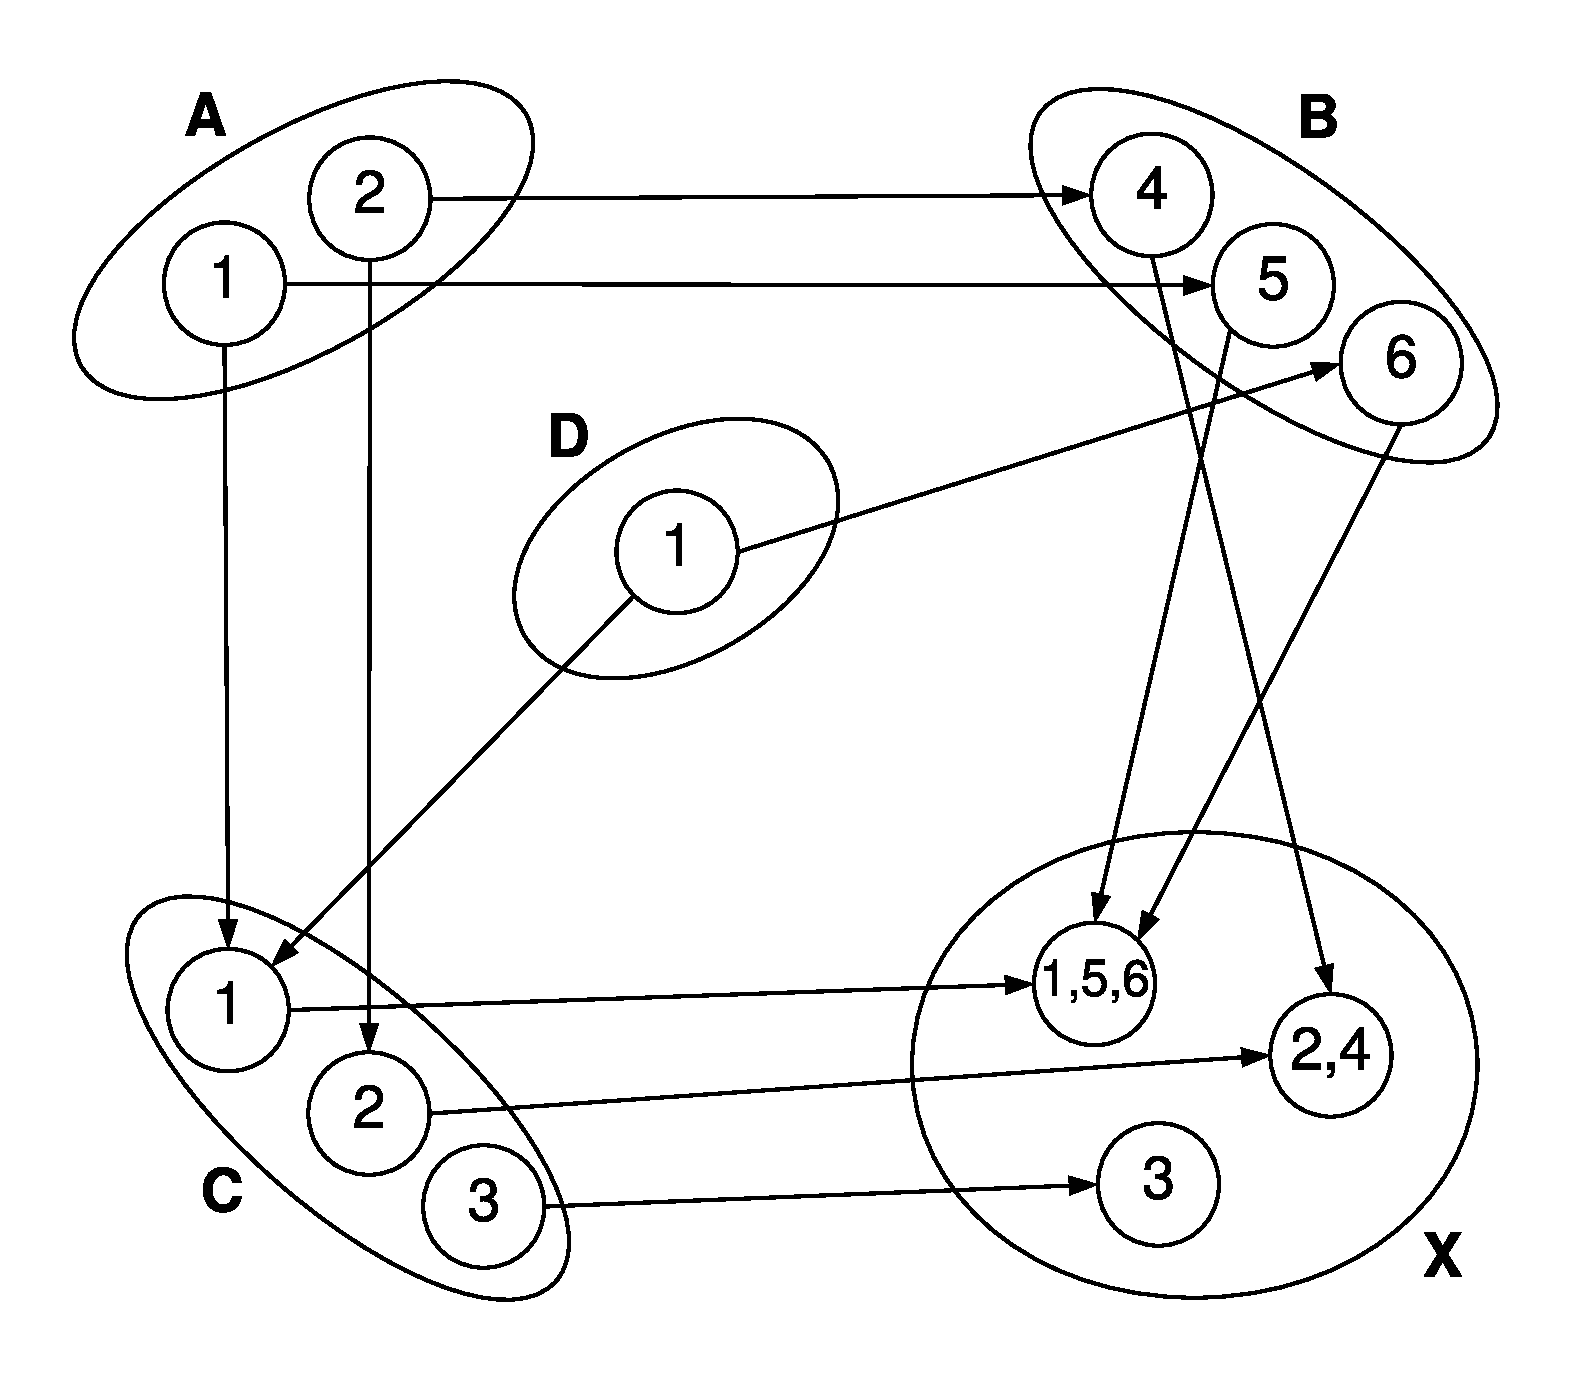
\includegraphics[scale=0.4]{images/gts/colimit}
  \caption{A colimit in \cat{Set}}\label{fig:gts:colimit}
\end{figure}

\end{example}


\iffalse
\begin{definition}[Pullback] \tinytodo{Maintain only if we are going to use the concurrent rules chapter} Given 

\diagram{
  X'\ar@{.>}[dr]^{!}\ar@/^1.1pc/[rrd]^{i}\ar@/_1.1pc/[ddr]_{j}  & &\\
  & X\ar[r]^{g'}\ar[d]_{f'} & B\ar[d]^{f}\\
  & C\ar[r]_{g}      & A
}
\end{definition}

\begin{example}[Pullbacks in \cat{Set}]
\end{example}
\fi

\section{Graph Grammars}

The theory of graph grammars and graph transformation systems is based on the application of rules that are able to modify graphs. Using this framework, it is possible to model complex systems as graph transformation systems, where graphs represent the system states and the rules model transitions between states.

Graph grammars have a wide application in computer science, not only because graphs are very natural and intuitive way to model complex situations, but also because it is possible to reason about several properties of the modelled systems using its formalism~\cite{Ehrig2006,Rozenberg1997}.

We now review the basic concepts and analysis techniques for graph transformations that are used in this work.

\begin{definition}[Graph] A graph is a tuple $G = \left(V,E,s,t\right)$ where: $V$ is a set of nodes, $E$ is a set of Edges and $s,t : E \rightarrow V$ are two total functions that map each edge in $E$ to its source and target in $V$.

\end{definition}

\begin{example}[Graph]\label{def:graph} Figure~\ref{fig:gts:graph} shows a simple graph $G$ with $V = \{1,2,3,4\}$, $E = \{1,2\}$, $s =\{(1,1),(2,3)\}$ and $t = \{(1,2),(2,3)\}$.
\begin{figure}[!ht]
  \centering
  
\includegraphics[scale=0.8]{images/gts/graph}
  \caption{A graph example}\label{fig:gts:graph}
\end{figure}
\end{example}

\begin{definition}[Graph Morphism]\label{def:graph-morphism} Given two graphs $G_1,G_2$ with \mbox{$G_i = \left(V_i, E_i, s_i, t_i\right)$} for $i$ in $[1,2]$, a graph morphism $f : G_1 \rightarrow G_2$ between them is a pair $f = \left(f_V,f_E\right)$ where $f_V : V_1 \rightarrow V_2$ and $f_E : E_1 \rightarrow E_2$ are total functions that preserve the source and target functions, i.e. $f_V \circ s_1 = s_2 \circ f_E$ and $f_V \circ t_1 = t_2 \circ f_E$.
\end{definition}

\begin{example}[Graph Morphisms]Figure~\ref{fig:gts:compact-graph-morphism} shows three morphisms $f : G_0 \rightarrow G_1$, $g : G_0 \rightarrow G_2$ and $h : G_0 \rightarrow G_3$, which are a monomorphism, an epimorphism and a isomorphism, respectively.

  The morphism $f$ maps node $\Circle_1$ to $\Circle_a$, node $\Circle_2$ to $\Circle_b$ and edge $\curvearrowleft_1$ to $\curvearrowleft_q$; $g$ maps both nodes $\Circle_1$ and $\Circle_2$ to $\Circle_c$ and edge $\curvearrowleft_1$ to $\curvearrowleft_r$; and $h$ maps node $\Circle_1$ to $\Circle_d$, node $\Circle_2$ to $\Circle_e$ and edge $\curvearrowleft_1$ to $\curvearrowleft_s$.

  Figure~\ref{fig:gts:expanded-graph-morphism} shows the morphism $f$ in an expanded (explicit) notation. Both notations will be used through this work, according to which one will be the better to clarify the meaning at the moment.
\begin{figure}[!ht]
  \centering
  \fbox{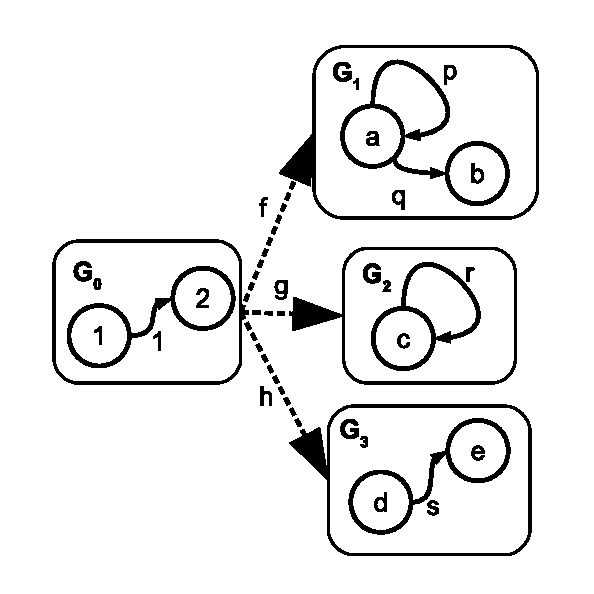
\includegraphics[scale=0.8]{images/gts/compact-graph-morphism}}
  \caption{A graph morphism example}\label{fig:gts:compact-graph-morphism}
\end{figure}

\begin{figure}[!ht]
  \centering
  \fbox{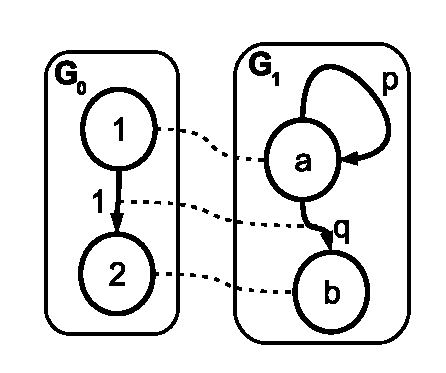
\includegraphics[scale=0.8]{images/gts/expanded-graph-morphism}}
  \caption{An expanded graph morphism example}\label{fig:gts:expanded-graph-morphism}
\end{figure}
\end{example}

\begin{definition}[Typed Graph and Typed Graph Morphism] A type graph is a distinguished graph $TG = \left(V_{TG},E_{TG},s_{TG},t_{TG}\right)$ where $V_{TG}$ and $E_{TG}$ are called the node and edge type alphabets, respectively.

  A typed graph is a pair $G^T = \left(G, type\right)$ consisting of a graph $G$ and a graph morphism $type : G \rightarrow TG$.

  Given two typed graphs $G^T_1 = \left(G_1,type_1\right)$ and $G^T_2 =\left(G_2,type_2\right)$, a typed graph morphism $f : G^T_1 \rightarrow G^T_2$ is a graph morphism $f : G_1 \rightarrow G_2$ such that $type_2 \circ f = type_1$:

\diagram{
  G_1\ar[rr]^{f}\ar[dr]_{type_1} & & G_2\ar[dl]^{type_2}\\
  \ar@{}[rur]|{=}& TG &
}
\end{definition}

\begin{example}[Typed Graph and Typed Graph Morphism Example] Figure~\ref{fig:gts:typed-graphs} shows a type graph $T$, and four graphs $G_0, G_1, G_2, G_3$ where only $G_0$ and $G_1$ are valid \emph{T-typed} graphs. 
  
  Notice that $G_2$ can not be a \emph{T-typed} graph because type graph does not have a node of the type $\lozenge$, neither an edge type with source and target in the $\Square$ type. Similarly, $G_3$ is not a valid \emph{T-typed} graph because, although there is an edge type between a $\triangle$ and a $\Square$ types, the source must of this type of edge must be a $\Square$ and the target a $\triangle$.

  Figure~\ref{fig:gts:typed-graph-morphism} shows a typed graph morphism $f : G_0^T \rightarrow G_1^T$, where $f$ maps node $\Circle_a$ to $\Circle_1$, $\Square_b$ to $\Square_1$ and edge $\curvearrowleft_e$ to $\curvearrowleft_2$.
\begin{figure}[!ht]
  \centering
  \fbox{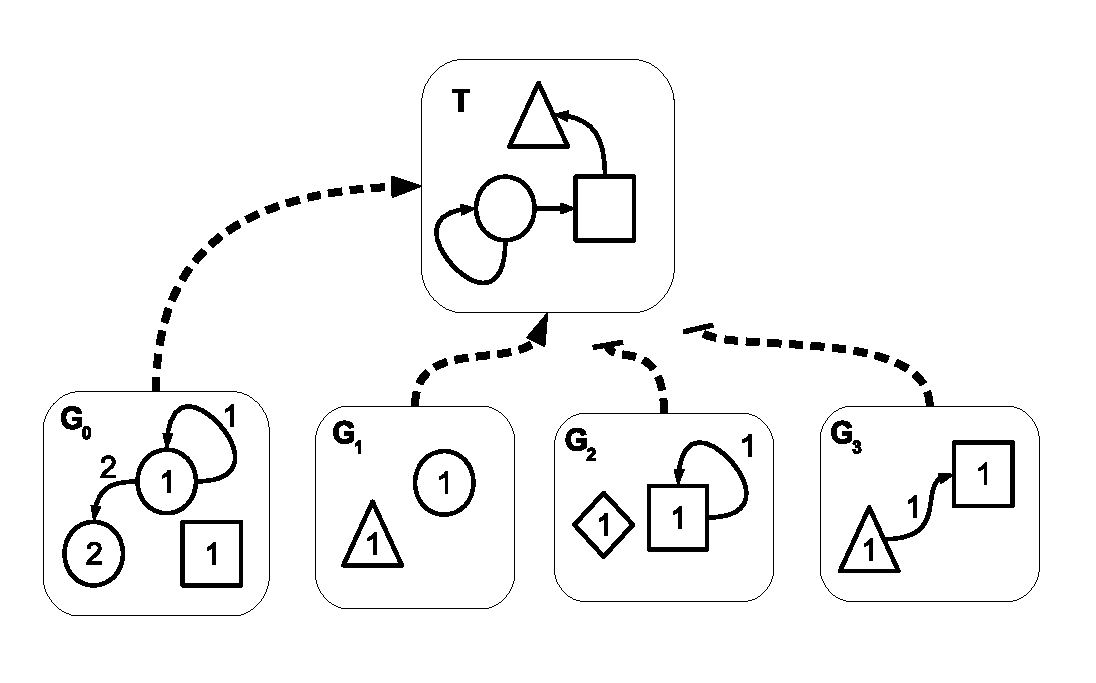
\includegraphics[scale=0.65]{images/gts/typed-graphs}}
  \caption{\emph{T-typed} valid and invalid graphs}\label{fig:gts:typed-graphs}
\end{figure}

\begin{figure}[!ht]
  \centering
  \fbox{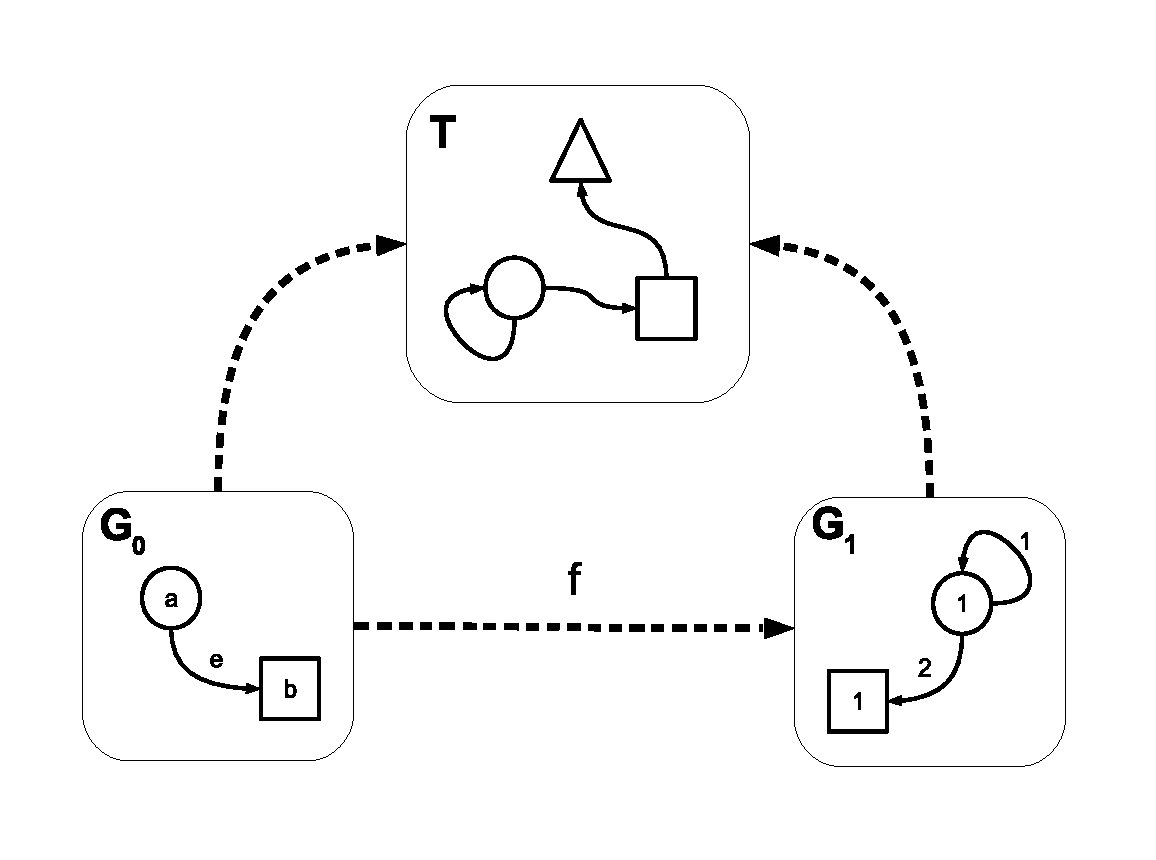
\includegraphics[scale=0.6]{images/gts/typed-graph-morphism}}
  \caption{A typed graph morphism}\label{fig:gts:typed-graph-morphism}
\end{figure}
\end{example}

\begin{remark}[Categories of Graphs and Typed Graphs] We call \cat{Graph} the category whose objects are graphs and arrows are graph morphisms. Similarly, we have that \cat{TGraph_T} is the category whose objects are $T-$typed graphs and whose arrows are $T-$typed graph morphisms.
\end{remark}

\iffalse
\begin{definition}[Positive Atomic Constraint] A \emph{positive} atomic (typed) graph constraint is of the form $PC\left(a\right)$, where $a : P \rightarrow C$ is a (typed) graph morphism. A (typed) graph $G$ satisfies $PC\left(a\right)$ if for every injective (typed) graph morphism $p : P \rightarrow G$ there is at least one injective (typed) graph morphism $q : P \rightarrow C$ such that $p = q \circ a$.

  A positive (typed) graph constraint with $a : \emptyset \rightarrow C$ is also notated $PC\left(C\right)$. Given a (typed) graph $G$, it satisfies $PC\left(C\right)$ if there is an injective (typed) graph morphism $q : C \rightarrow  G$.
\diagram{
  P\ar[rr]^{a}\ar[dr]_{p} & & C\ar[dl]^{q}\\
  \ar@{}[rur]|{=}& G &
}

\end{definition}

\begin{definition}[Negative Atomic Constraint]
A \emph{negative} atomic (typed) graph constraint is of the form $NC\left(a\right)$, where $a : P \rightarrow C$ is a (typed) graph morphism. A (typed) graph $G$ satisfies $PC\left(a\right)$ if for every injective (typed) graph morphism $p : P \rightarrow G$ there is no injective (typed) graph morphism $q : P \rightarrow C$ such that $p = q \circ a$.

  A negative (typed) graph constraint with $a : \emptyset \rightarrow C$ is also notated $NC\left(C\right)$. Given a (typed) graph $G$, it satisfies $NC\left(C\right)$ if there is no injective (typed) graph morphism $q : C \rightarrow G$.

\diagram{
  P\ar[rr]^{a}\ar[dr]_{p} & & C\ar[dl]|{|}^{q}\\
  \ar@{}[rur]|{=}& G &
}

\end{definition}

\begin{remark} It was shown in ~\cite{Ehrig2006} that negative atomic constraints do not give more expressive power. However, we introduced this concept because it makes easier to reason about some of the purposes of this thesis in a negative rather than a positive manner.%\tinytodo{related to the graph constraint definition, maybe this is not necessary}
\end{remark}

\begin{definition}[Graph Constraint] A (typed) graph constraint is a \emph{boolean} formula over atomic (typed) graph constraints, in such way that $true$, $false$ and every atomic constraint are also graph constraints. Also, if $c$ and $c_i$, with $i \in I$ for some index set $I$, are graph constraints, then $\neg c$, $\land_{i \in I} c_i$ and $\lor_{i \in I} c_i$ are also graph constraints.

  A graph $G$ satisfies a graph constraint $c$ (written $G \models c$) iff one of the following situations occurs:
  \begin{itemize}
    \item $c = true$
    \item $c$ is an atomic constraint $a$ and $G \models a$
    \item $c = \neg c'$ and $G \not\models c'$
    \item $c = \land_{i \in I}c_i$ and $G \models c_i$ $\forall i \in I$ 
    \item $c = \lor_{i \in I}c_i$  and $\exists i \in I$ such that $G \models c_i$
  \end{itemize}
\end{definition}

\begin{example}[Constraints Example]
\end{example}
\fi

\begin{definition}[Graph Rule]\label{def:graph-rule} A (typed) graph rule\footnote{Also called graph transformation rule or graph production.} \graphrule{} is a span of (typed) graph monomorphisms \lefthand{} and \righthand{}  where the (typed) graphs $L$, $K$ and $R$ are called the left-hand side, gluing graph and right-hand side, respectively.

  Given a (typed) graph rule $p$, its inverse rule is defined by \inversegraphrule.
\end{definition}

\begin{example}[Graph Rule Example and Notation] Figure~\ref{fig:gts:rule} shows an example of a graph rule which reads a node of the type $\Circle$, deletes a node of the type $\triangle$ and then creates a node of the type $\Square$ with an edge between the $\Circle$ and the \Square. 
  
Figure~\ref{fig:gts:rule-standard} presents the rule in the standard DPO notation, while Figure~\ref{fig:gts:rule-compact} depicts the same rule in a compact notation, where the gluing graph is omitted. 

Sometimes we will use the compact notation to make the figures smaller. Notice that the compact notation does not cause any semantic loss as the gluing graph can be obtained as the ``intersection'' between the left and right graphs, and the morphisms $l$ and $r$ as the inclusions of $K$ in $L$ and $R$, respectively.

\begin{figure}[!ht]
  \centering
  \begin{subfigure}[t]{.5\textwidth}
    \centerline{\fbox{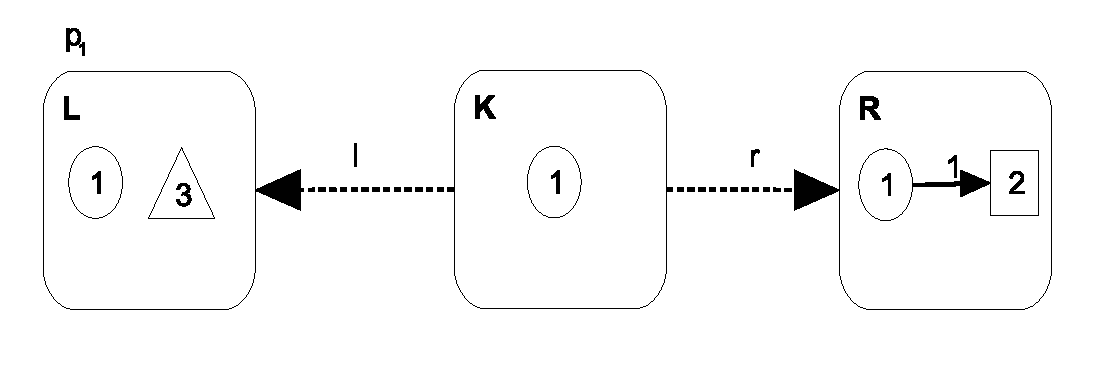
\includegraphics[scale=0.5]{images/gts/standard-dpo-rule}}}
    \caption{Standard DPO rule notation}\label{fig:gts:rule-standard}
  \end{subfigure}

  \begin{subfigure}[t]{.5\textwidth}
    \centerline{\fbox{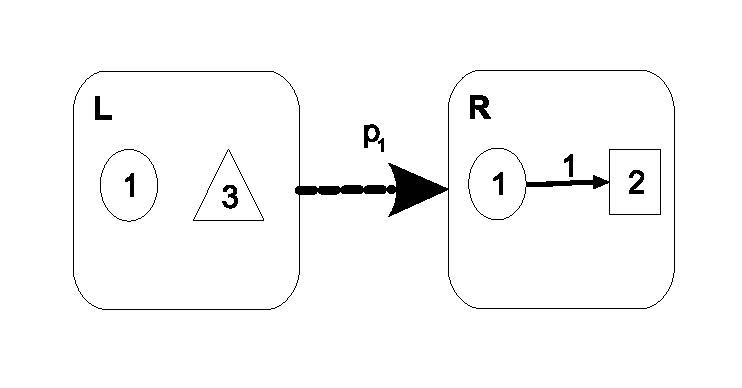
\includegraphics[scale=0.5]{images/gts/compact-dpo-rule}}}
    \caption{Compact DPO rule notation}\label{fig:gts:rule-compact}
  \end{subfigure}
  \caption{DPO graph rule}\label{fig:gts:rule}
\end{figure}
\end{example}

\begin{definition}[Graph Transformation] Given a (typed) graph rule \graphrule{} and a (typed) graph $G$ with a (typed) graph morphism \match, called match, a direct (typed) graph transformation $G \xRightarrow{p,m} H$ from $G$ to a (typed) graph $H$ is a double-pushout (DPO) diagram such as:

\diagram{
  L\ar[d]_{m}        & & K\ar[ll]_{l}\ar[rr]^{r}\ar[d]|{k} & & R\ar[d]^{m'}\\
  G\ar@{}[urr]|{\left(1\right)} & & D\ar[ll]^{f}\ar[rr]_{g}             & & H\ar@{}[ull]|{\left(2\right)}
}

  For \cat{TGraph_T} there are two conditions, called \emph{gluing conditions}, that must be satisfied so that the pushouts (1) and (2) exist and the rule graph rule can be applied:
  
  First, the \emph{dangling condition} requires that no node can be deleted if it has incident edges that are not also deleted (otherwise the result of this deletion would not be a graph).  Second, the \emph{identification condition} requires the match to not identify a deleted element with a preserved or (another) deleted one.
\end{definition}

\begin{example}[Graph Transformation Examples] Figure~\ref{fig:gts:transformation-success} shows a transformation where the rule depicted in Figure~\ref{fig:gts:rule} is successfully applied over a graph instance $G_0$.

  Figure~\ref{fig:gts:transformation-fail} shows the same rule being applied over a graph instance $G_1$ which does not satisfy the gluing conditions, more specifically it does not satisfy the dangling condition.

\begin{figure}[!ht]
  \centering
  \begin{subfigure}[t]{.5\textwidth}
    \centerline{\fbox{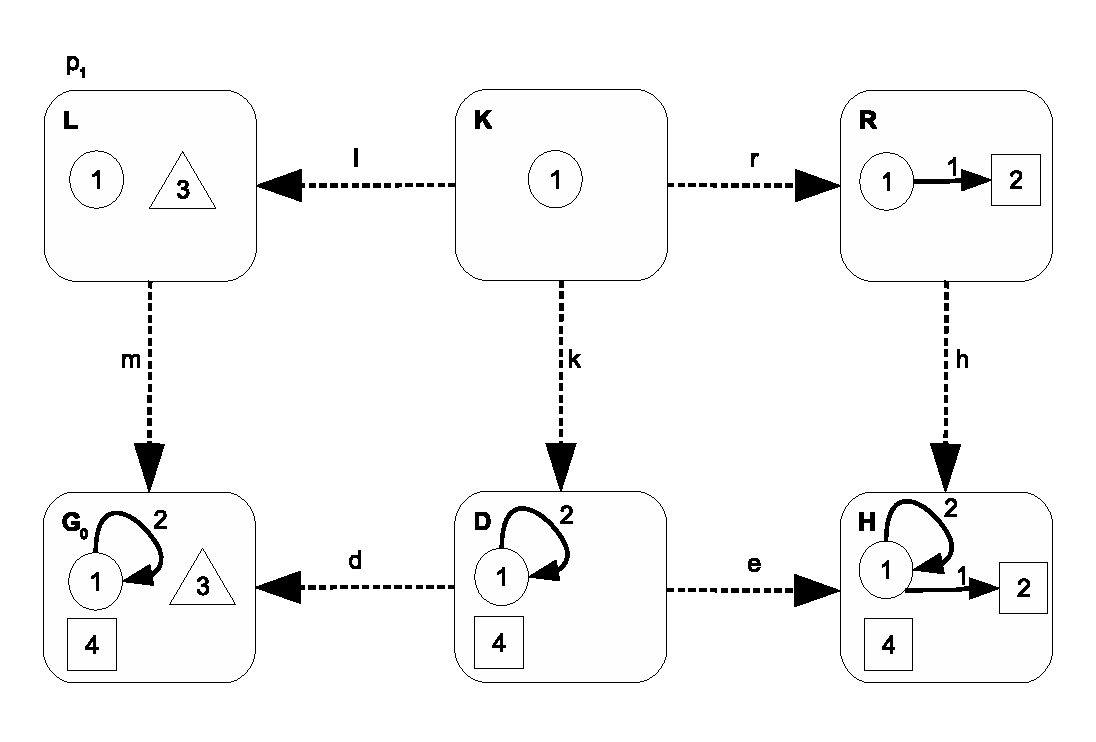
\includegraphics[scale=0.8]{images/gts/transformation}}}
    \caption{Successfully applied graph transformation}\label{fig:gts:transformation-success}
  \end{subfigure}

  \begin{subfigure}[t]{.5\textwidth}
    \centerline{\fbox{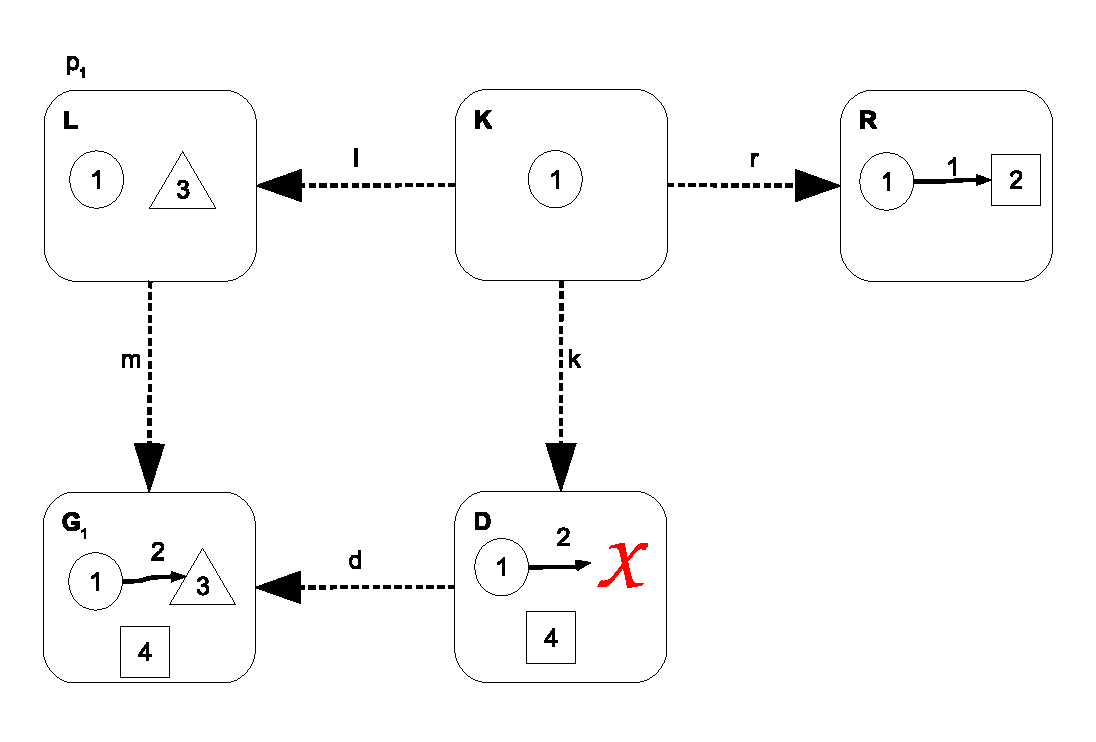
\includegraphics[scale=0.8]{images/gts/transformation-failed}}}
    \caption{Failing graph transformation due to the dangling condition}\label{fig:gts:transformation-fail}
  \end{subfigure}
  \caption{Graph transformation}\label{fig:gts:transformation}
\end{figure}

\end{example}
\begin{definition}[Negative Application Condition] A \emph{left} negative application condition over a graph rule \graphrule{} is of the form $NAC\left(n\right)$, where \nac{} is an arbitrary (typed) graph morphism. A match \match{} of a rule $p$ satisfies\footnote{When a NAC is satisfied it is also said that the NAC is \emph{not triggered} and vice versa.} $NAC\left(n\right)$ on $L$, written $m \models NAC\left(n\right)$, iff $\nexists$ $q : N \rightarrow G$ with $q$ injective and $q \circ n = m$.

\diagram{
  N\ar@{.>}[dr]|{|}_{q} & L\ar[d]^{m}\ar[l]_{n}\\
   & G
}

  A match \match{} satisfies a set \mbox{$NAC_L = \{NAC\left(n_i\right)|i \in I\}$} of left $NACs$, iff \mbox{$m \models NAC\left(n_i\right)$} $\forall i \in I$.

  Analogously, a \emph{right} negative application condition over a graph rule \graphrule{} is of the form $NAC\left(n\right)$, where \rightnac{} is an arbitrary (typed) graph morphism. A comatch \comatch{} of a rule $p$ satisfies $NAC\left(n\right)$ on $R$ (written \mbox{$m' \models NAC\left(n\right)$}) iff $\nexists$ $q : N \rightarrow H$ with $q$ injective and $q \circ n = m'$.

\diagram{
  R\ar[d]_{m'}\ar[r]^{n} & N\ar@{.>}[dl]|{|}^{q}\\
  H &
}
  Also, a comatch \comatch{} satisfies a set \mbox{$NAC_R = \{NAC\left(n_i\right)|i \in I\}$} of right $NACs$, iff $m' \models NAC\left(n_i\right)$ $\forall i \in I$.

\end{definition}

\begin{example}[NAC and NAC satisfiability] Figure~\ref{fig:gts:nacs:satisfied} shows a NAC that is satisfied (i.e. not triggered) over a match $m$, as there is no possible way of mapping the edge between $\Circle_1$ and $\Square_1$ in $N$ to an edge in $G_0$ such that the resulting triangle commutes. Therefore, if $G_0$ also satisfies the gluing conditions for the corresponding rule the transformation can be applied.

  On the other hand, Figure~\ref{fig:gts:nacs:triggered} shows a NAC that is triggered (i.e. not satisfied) over the match $m$: all the elements in $N$ can be mapped to $G_0$ such that the resulting triangle commutes. Therefore, even if $G_0$ satisfies the gluing conditions, the transformation can not be applied, as the pattern forbidden by the NAC was found on the instance graph.

\begin{figure}[!ht]
  \centering
  \begin{subfigure}[t]{.5\textwidth}
    \centerline{\fbox{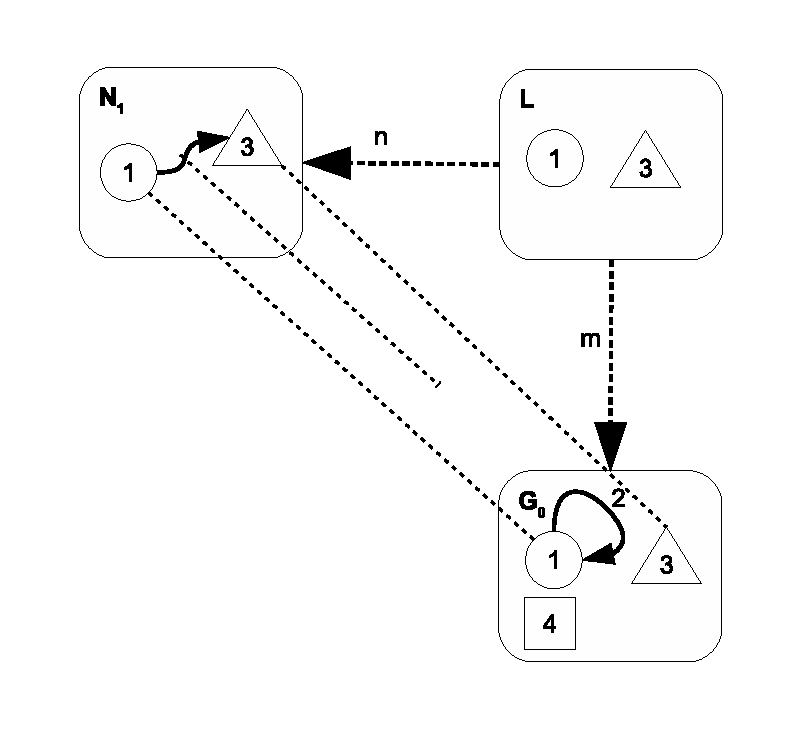
\includegraphics[scale=0.55]{images/gts/satisfied_nac}}}
    \caption{A satisfied NAC}\label{fig:gts:nacs:satisfied}
  \end{subfigure}%
  \begin{subfigure}[t]{.5\textwidth}
    \centerline{\fbox{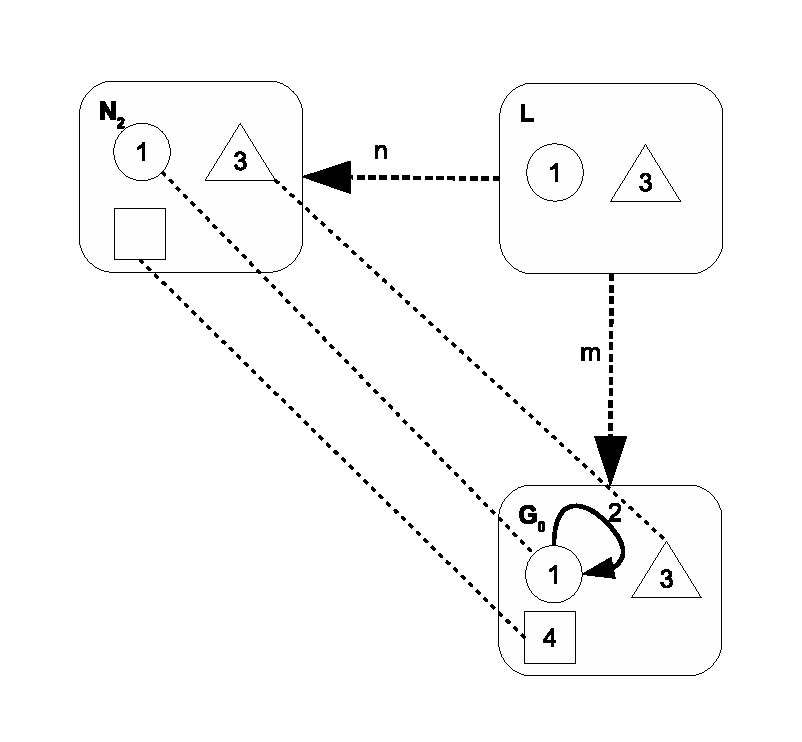
\includegraphics[scale=0.55]{images/gts/triggered_nac}}}
    \caption{A triggered NAC}\label{fig:gts:nacs:triggered}
  \end{subfigure}
  \begin{subfigure}[t]{.5\textwidth}
    \centerline{\fbox{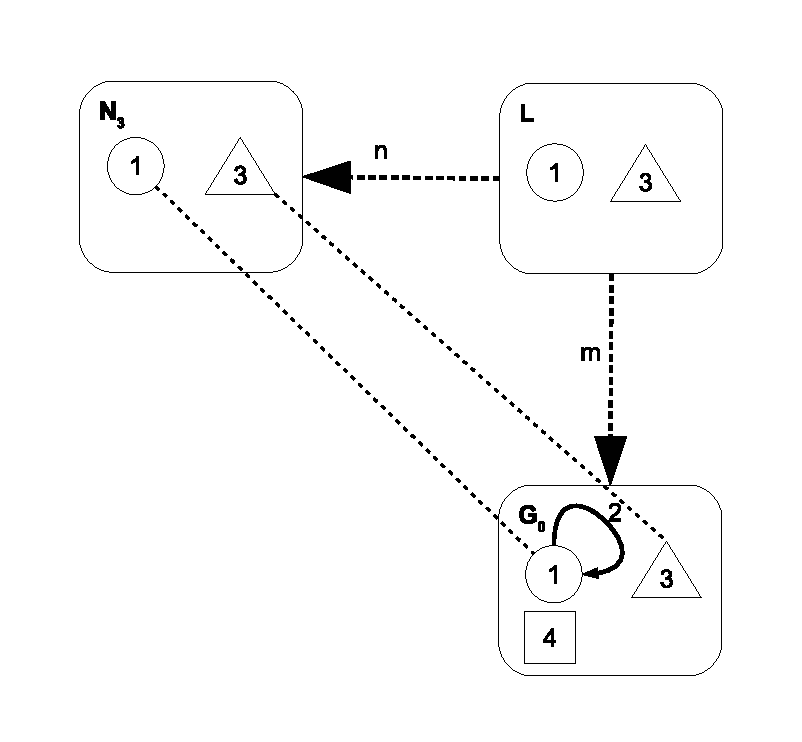
\includegraphics[scale=0.55]{images/gts/trivially_triggered_nac}}}
    \caption{A trivially-triggered NAC}\label{fig:gts:nacs:trivial}
  \end{subfigure}
  \caption{NACs and NAC satisfiability}\label{fig:gts:nacs}
\end{figure}
\end{example}

%\begin{assumption}[Left NACs] Unless stated otherwise, we will work with graph rules that have only left $NACs$ for the rest of this thesis. This is without loss of generality once right $NACs$ can be translated to left ones as it is shown in Definition~\ref{def:shift-nac}.
%\end{assumption}

\begin{definition}[Trivially-Triggered NACs] Given a $NAC(n)$, where $n : L \rightarrow \hat{L}$ is a isomorphism, and a match \match{} which is also a monomorphism, we call $NAC(n)$ a \emph{trivially-triggered NAC} as, for every monomorphic $m$, there will always exist a $q : \hat{L} \rightarrow G$ injective such that $q \circ n = m$.

  A trivially-triggered NAC $n : L \rightarrow \hat{L}$ is also notated $NAC(L)$. If a rule $p$ has a trivially-triggered NAC then $p$ can never be applied whatsoever, as the NAC will never be satisfied. An example of a trivially-triggered NAC is shown on Figure~\ref{fig:gts:nacs:trivial}.
\end{definition}

\begin{definition}[Graph Transformation System and Graph Grammar] A typed graph transformation system is a pair $GTS = \left(TG,P\right)$ where $TG$ is the type graph of the system and $P$ is a set of typed graph rules with NACs.

  A typed graph grammar is a pair $GG = \left(GTS,I\right)$ where $TGS$ is a typed graph transformation system and $I$ is a typed start graph. It can also be notated as $GG = \left(TG, I^{TG},P \right)$.

\end{definition}

\begin{example}[Mail Server Graph Transformation System] Fig~\ref{fig:gts:mail} depicts a graph transformation system that models a client-server scenario for a very simple e-mail application. This system has only four actions: 

\begin{enumerate}
  \item \emph{sendMessage}: a client sends a message to a server,\tinytodo{fix arrow direction}
  \item \emph{getData}: a piece of data is obtained from a server,
  \item \emph{receiveMessage}: a server sends a message to a client,
  \item \emph{deleteMessage}: a client obtains a piece of data from a received message and the message is destroyed.
\end{enumerate}

\begin{figure}[!ht]
  \centering
  \begin{subfigure}[t]{.5\textwidth}
    \centerline{\fbox{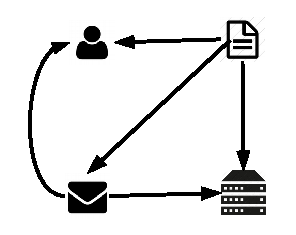
\includegraphics[scale=0.5]{gts/grammar/grammar-type-graph}}}
    \caption{Type Graph}
  \end{subfigure}
  \begin{subfigure}[t]{.5\textwidth}
    \centerline{\fbox{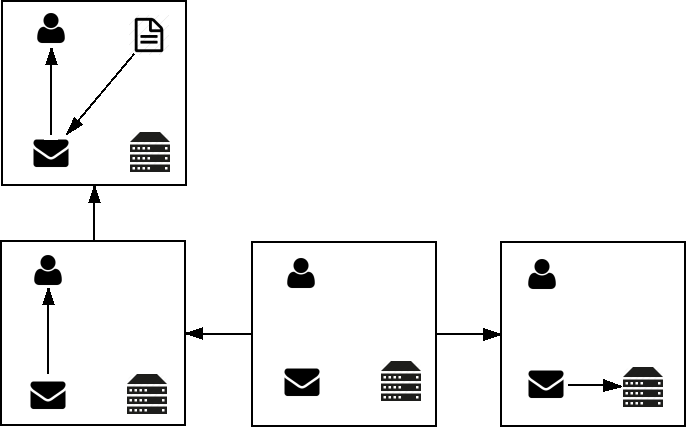
\includegraphics[scale=0.3]{gts/grammar/sendMessage}}}
    \caption{Send message}
  \end{subfigure}%
  \begin{subfigure}[t]{.5\textwidth}
    \centerline{\fbox{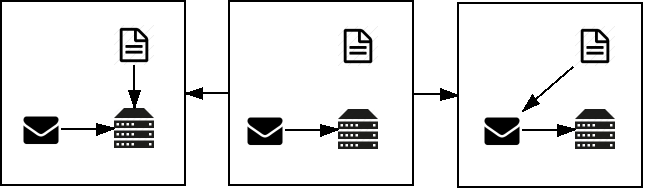
\includegraphics[scale=0.3]{gts/grammar/getData}}}
    \caption{Get data}
  \end{subfigure}
  \begin{subfigure}[t]{.5\textwidth}
    \centerline{\fbox{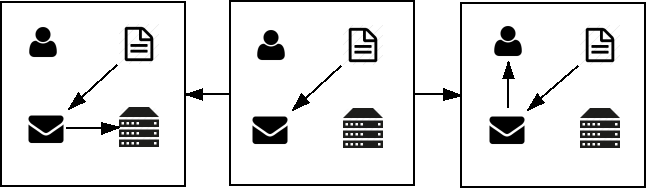
\includegraphics[scale=0.3]{gts/grammar/receiveMessage}}}
    \caption{Receive message}
  \end{subfigure}%
  \begin{subfigure}[t]{.5\textwidth}
    \centerline{\fbox{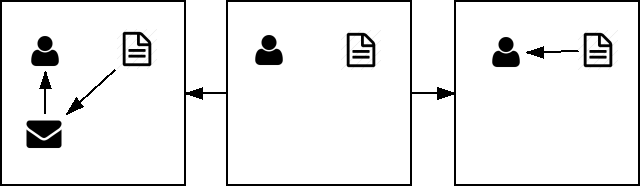
\includegraphics[scale=0.3]{gts/grammar/deleteMessage}}}
    \caption{Delete message}
  \end{subfigure}
  \caption{Mail application graph transformation system}\label{fig:gts:mail}
\end{figure}

\iffalse
\begin{figure}
\centering
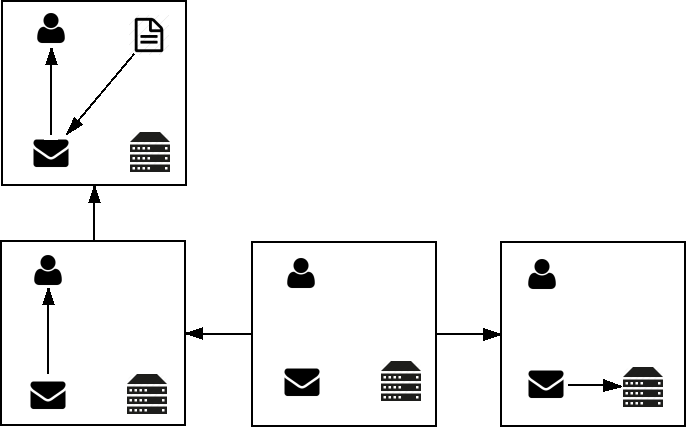
\includegraphics[width=6.5cm]{gts/grammar/sendMessage}
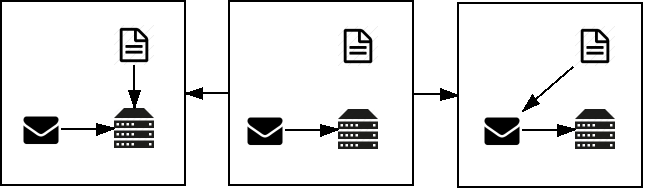
\includegraphics[width=5cm]{gts/grammar/getData}
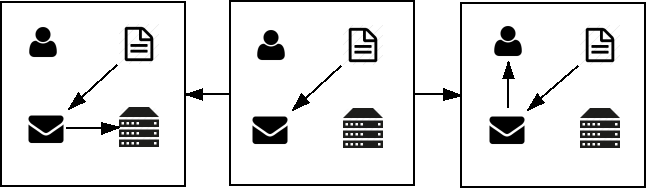
\includegraphics[width=5cm]{gts/grammar/receiveMessage}
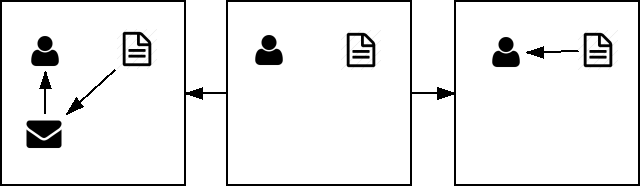
\includegraphics[width=5cm]{gts/grammar/deleteMessage}
\caption{\label{fig:gts:mail} Graph rules for Server}
\end{figure}
\fi
\end{example}

\section{Parallel and Sequential Independence}

One of the characteristics that make Graph Transformation Systems and Graph Grammars suitable formalisms to model and reason about parallel and/or concurrent systems is the possibility to check whether the transformations given by two graph rules over the same instance graph can be applied (1) at the same time or (2) in any interchangeable order. In the first case we say that the transformations are parallel independent; in the later we say that they are sequential independent.

In this section, we show both what it means for two graph transformations to be independent and how to check it. Notice that when we are reasoning about graph transformations the (in)dependence is concrete, while for the case of graph rules the (in)dependence is potential, as it would depend on a particular pattern being found on an instance graph.

\begin{definition}[Causal Dependency]\label{def:classic-dependency} Given two graph rules $p_1,p_2$ with NACs, they are \emph{causally dependent} for a given graph $E$, in which they overlap, iff one of the following situations occurs in the transformations diagram:

  \begin{enumerate}
    \item $\nexists h_{12} : R_1 -> D_2$ such that $d_2 \circ h_{12} = m_1'$
    \item $\exists! h_{12} : R_1 -> D_2$ such that $d_2 \circ h_{12} = m_1'$ but $e_2 \circ h_{12} \not\models NAC_{p_1^{-1}}$
    \item $\nexists h_{21} : L_2 -> D_1$ such that $e_1 \circ h_{21} = m_2$
    \item $\exists! h_{21} : L_2 -> D_1$ such that $e_1 \circ h_{21} = m_2$ but $d_1 \circ h_{21} \not\models NAC_{p_2}$
  \end{enumerate}

\diagram{
    N_1 & & & & N_2 & & \\
      L_1\ar[d]\ar[u]^{n_1} & K_1\ar[d]\ar[l]\ar[r] & R_1\ar[dr]_{m'_{1}}\ar@{.>}@/^1.1pc/[drrr]|<<{|}^<<<{h_{12}} & & L_2\ar[dl]^{m_2}\ar[u]^{n_2}\ar@{.>}@/_1.1pc/[dlll]|<<{|}_<<<{h_{21}} & K_2\ar[d]\ar[l]\ar[r] & R_2\ar[d]\\
        H_1 & D_1\ar[l]^{d_1}\ar[rr]_{e_1} & & \textit{E} & & D_2\ar[ll]^{d_2}\ar[r]_{e_2} & H_2\\
          & & & & & &
          }
\end{definition}

Intuitively, each case of dependency can be regarded as follows:

\begin{enumerate}
  \item a \emph{deliver-delete} dependency: $p_2$ deletes (from graph $E$) at least one element that was created or preserved by $p_1$.
  \item a \emph{forbid-produce} dependency: $p_2$ creates on $H_2$ at least one element that would trigger the NAC $N_1^{-1}$.
  \item a \emph{produce-use} dependency: $p_1$ creates (on graph $E$) at least one element needed for $p_2$ to be applied which did not exist on $H_1$.
  \item a \emph{delete-forbid} dependency: $p_1$ deletes (from graph $H_1$) at least one element that would trigger the NAC $N_2$, thus allowing the application of $p_2$ on $E$.
\end{enumerate}

\begin{example}[Dependency situation in the mail server grammar]
  Figure~\ref{fig:gts:dependency} shows a dependency situation between the rules \emph{getData} and \emph{receiveMessage}. In this case, the dependency is of a \emph{produce-use} kind: the edge between the \emph{piece of data} and the \emph{message} at the instance graph was created by \emph{getData} and the same edge is necessary for \emph{receiveMessage} to be applied.

\begin{figure}[!ht]
  \centering
  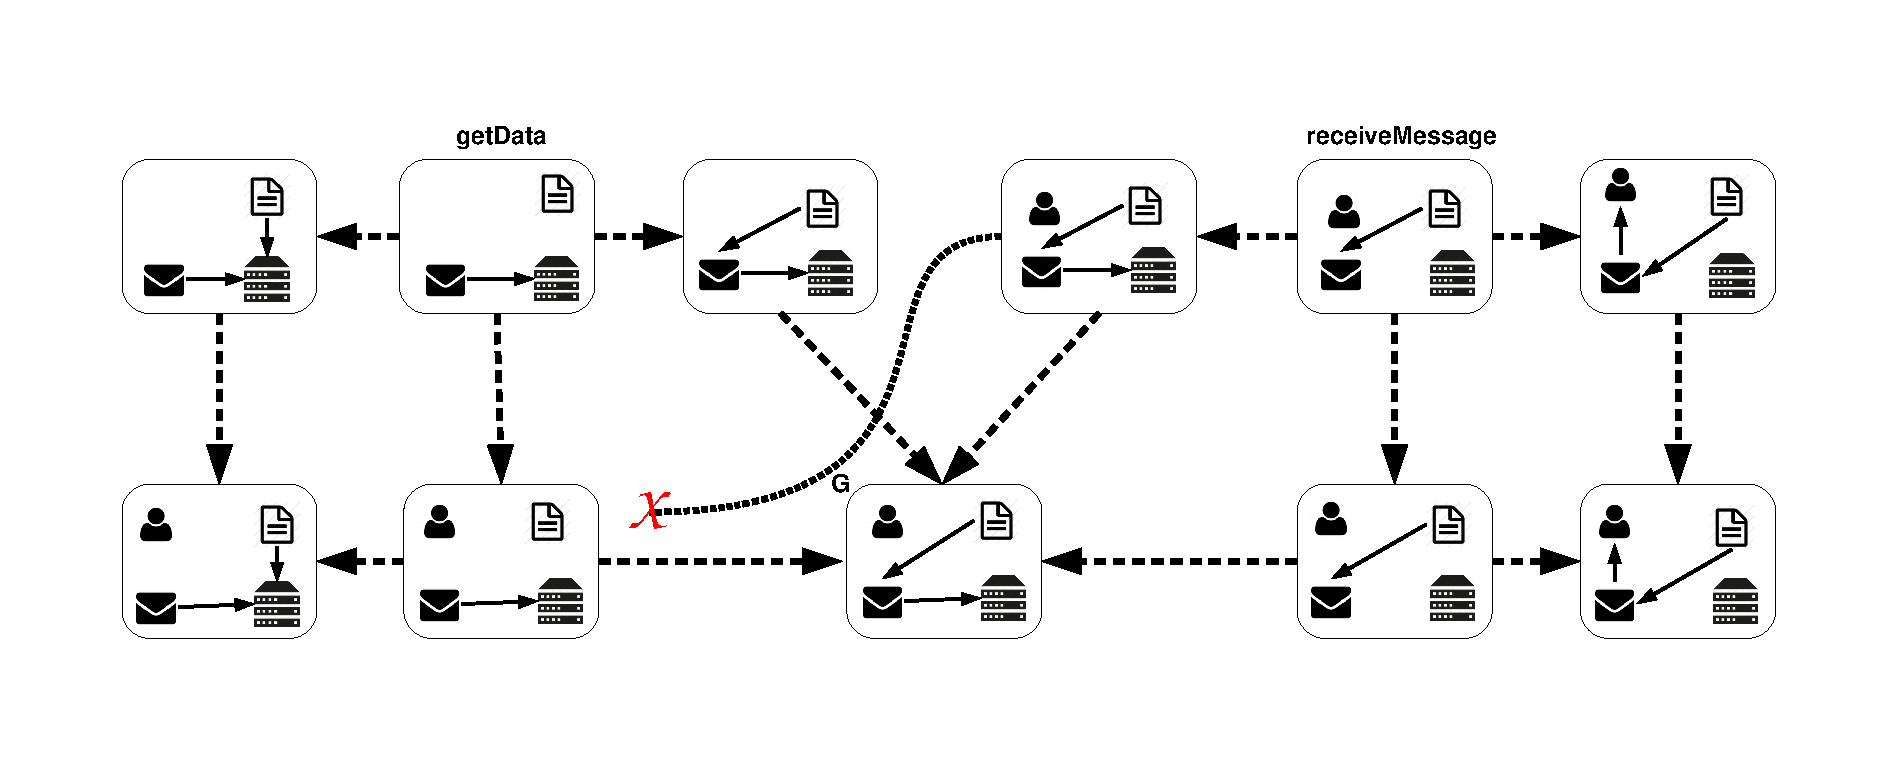
\includegraphics[scale=0.5]{images/gts/dependency}
  \caption{A dependency in the server grammar}\label{fig:gts:dependency}
\end{figure}

  In the diagram, it is not possible to find a morphism from the left-hand-side of \emph{receiveMessage} to the gluing graph of \emph{getData} such that the transformation is still valid. Thus, for the overlapping in this particular graph, \emph{receiveMessage} is causally dependent on \emph{getData}.
\end{example}

\begin{definition}[Conflict]\label{def:classic-conflict} Given two graph rules $p_1, p_2$ with NACs they are in conflict for a given graph $E$ in which they overlap iff one of the following situations occur:

\begin{enumerate}
    \item $\nexists h_{12} : L_1 -> D_2$ such that $d_2 \circ h_{12} = m_1$
    \item $\exists! h_{12} : R_1 -> D_2$ such that $d_2 \circ h_{12} = m_1$ but $e_2 \circ h_{12} \not\models NAC_{p_1}$
    \item $\nexists h_{21} : L_2 -> D_1$ such that $d_1 \circ h_{21} = m_2$
    \item $\exists! h_{21} : L_2 -> D_1$ such that $d_1 \circ h_{21} = m_2$ but $e_1 \circ h_{21} \not\models NAC_{p_2}$
  \end{enumerate}

\diagram{
     & & N_1 & & N_2 & & \\
      R_1\ar[d] & K_1\ar[d]\ar[l]\ar[r] & L_1\ar[u]^{n_1}\ar[dr]^{m_1}\ar@{.>}@/^1.1pc/[drrr]|<<{|}^<<<{h_{12}} & & L_2\ar[dl]_{m_2}\ar[u]^{n_2}\ar@{.>}@/_1.1pc/[dlll]|<<{|}_<<<{h_{21}} & K_2\ar[d]\ar[l]\ar[r] & R_2\ar[d]\\
        H_1 & D_1\ar[l]^{e_1}\ar[rr]_{d_1} & & \textit{E} & & D_2\ar[ll]^{d_2}\ar[r]_{e_2} & H_2\\
          & & & & & &
          }
\end{definition}

Intuitively, each conflict case can be regarded as:

\begin{enumerate}
  \item a \emph{delete-use} conflict: $p_2$ deletes (from graph $E$) at least one element needed for $p_1$ to be applied.
  \item a \emph{produce-forbid} conflict: $p_2$ produces (on graph $H_2$) at least one element that triggers the NAC $N_1$.
  \item a \emph{delete-use} conflict: $p_1$ deletes at least one element needed for $p_2$ to be applied
  \item a \emph{produce-forbid} conflict: $p_1$ creates at least one element that triggers the NAC $N_2$.
\end{enumerate}

\begin{example}[Conflict situation in the mail server grammar]
  Figure~\ref{fig:gts:dependency} shows a conflict situation involving the rules \emph{getData} and \emph{receiveMessage}. This is a \emph{delete-use} conflict: \emph{receiveMessage} deletes from the overlapping graph an edge between the \emph{message} and the \emph{server} which is necessary for \emph{getData} to be applied.

\begin{figure}[!ht]
  \centering
  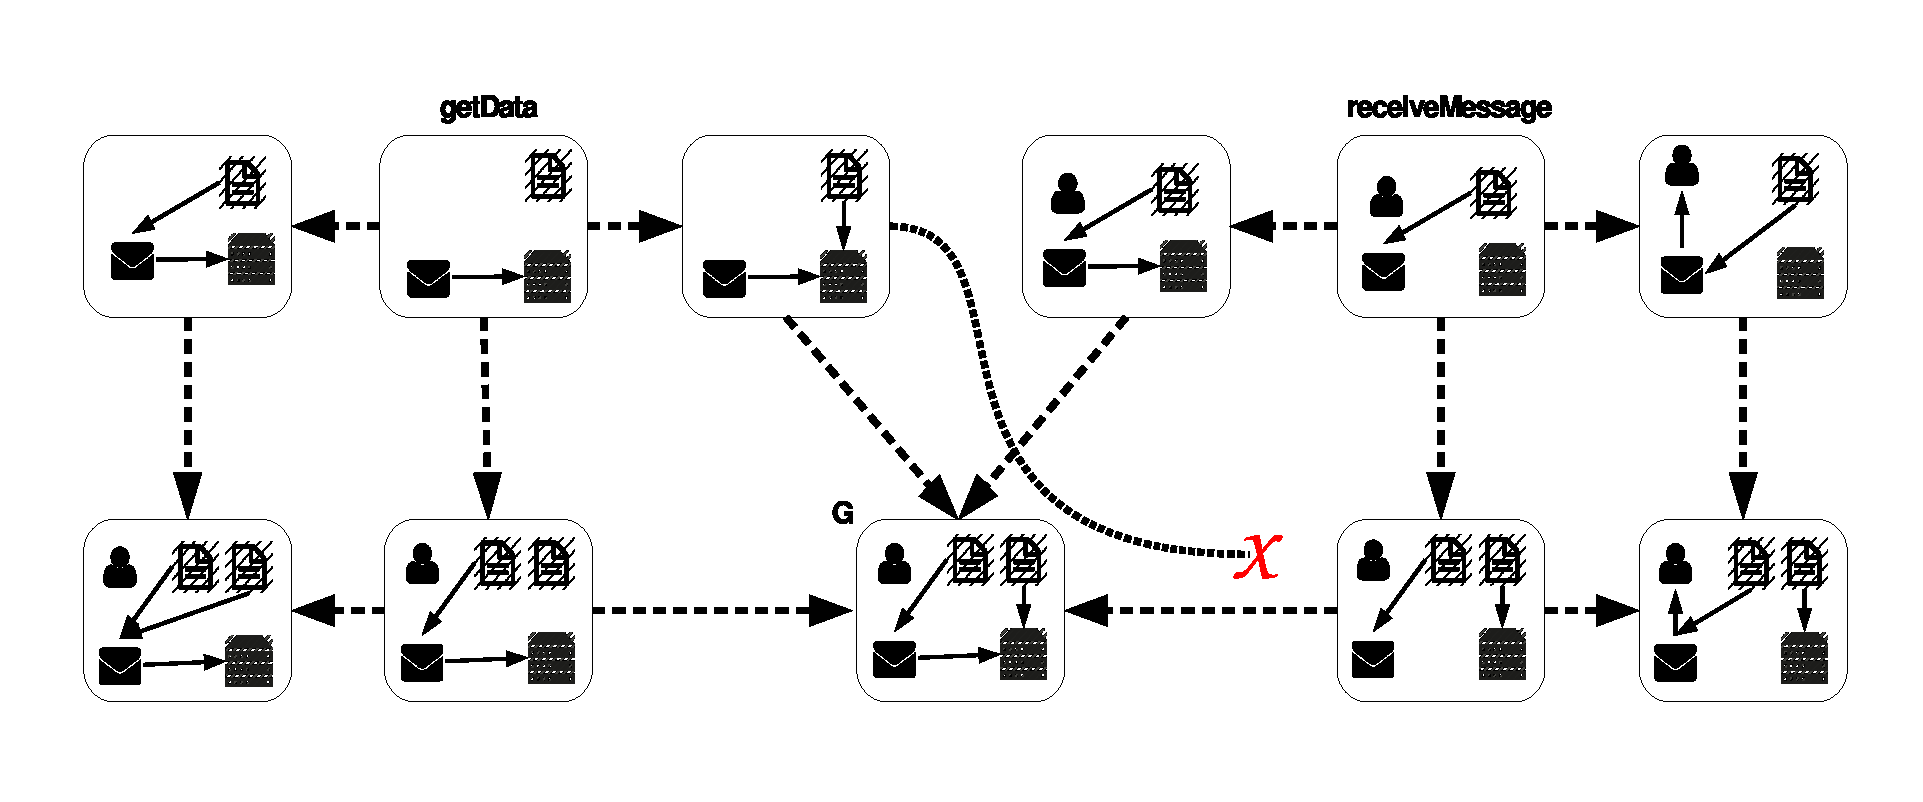
\includegraphics[scale=0.5]{images/gts/conflict}
  \caption{A conflict in the server grammar}\label{fig:gts:conflict}
\end{figure}

  Both rules are applied over the same graph and, individually, both transformations are valid. However, once \emph{receiveMessage} is applied, it is no longer possible to apply \emph{getData}. Represented in the diagram by the fat that it is not possible to find a morphism from the left-hand-side of \emph{getData} to the gluing graph of \emph{receiveMessage} such that the transformation from there is still valid.
\end{example}

  \chapter{Attributes}

Comparison between different kinds of implementation

\section{Concepts related to the Category of Algebras}

\section{Modelling attributes as F-Algebras?}

  \chapter{Concurrent Rules}

\section{Motivation}

What kind of concurrent rule do we expect and why?

Used in ~\cite{BezerraWEIT2016} and implemented in ~\cite{BezerraETMF2016}

\textbf{From the paper}

Given its formalism, there are several analysis techniques that can be performed over a Graph Grammar, including the \emph{concurrent rule} construction, which can be used to summarize the application of a sequence of several rules in one single step.

Graph Grammars that represent real systems usually have a considerable number of rules, possibly making it difficult to the modeller to foresee all possible rule interactions. Therefore it is important to have analysis techniques to address this issue, as well as tools that implement them.

We said earlier that the aim of calculating the concurrent rules is to summarize the combined effects of applying the transformations induced by a sequence of graph rules. Here we present how this can be done.

A \emph{rule sequence} is a list containing rules of a grammar in an specific order in which the modeller wants them to be applied. Given a rule sequence \mbox{$r =$ \rulesequence}, the construction of its correspondents concurrent rules is done by recursively combining pairs of subsequent rules, where the pairwise combination is defined as follows~\cite{Ehrig2006,Lambers2010}:  

\section{Concurrent Rules}

\begin{definition}[Concurrent Rules]

\diagram{
  L_c\ar[d]\ar\ar@{}[dr]|{(3)} & K_c\ar[d]\ar[l]\ar[r] \ar@{}[dr]|{(1)} & R_c\ar[dr]^{e_1} & & L_n\ar[dl]_{e_2} & K_n\ar[d]\ar[l]\ar[r]\ar@{}[dl]|{(2)} & R_n\ar[d]\ar@{}[dl]|{(4)}\\
  L & C_c\ar[l]^{c_l}\ar[rr]_{c_r} & & \textit{E} & & C_n\ar[ll]^{n_l}\ar[r]_{n_r} & R\\
  & & & K\ar@{.>}@/1pc/[llu]^{k_c}\ar@{.>}@/1pc/[urr]_{k_n}\ar@{}[u]|{(5)} & & &
}
\end{definition}

\begin{definition}[Downward Shifted NACs]

\diagram{
  N'_j\ar@{.>}@/0.5pc/[r]^{e_{ji}} & N_i\ar@{}[dl]|{=}\\
  A\ar[r]_{m}\ar[u]^{n'_j} & B\ar[u]_{n_i}
}

For each $NAC(n'_j)$ on $A$ with $n'_j : A \rightarrow N'_j$ and $m : A \rightarrow B$, 
let $D_m(NAC(n'_j)) = \{ NAC(n_i)|i \in I, n_i : B \rightarrow N_i \}$ where $I$ and $n_i$ 
are constructed as follows:
\begin{itemize}
  \item $i \in I$ iff $(e_{ji}, n_i)$ with $e_{ji} : N'_j \rightarrow N_i$ jointly surjective 
  \item $e_{ji} \circ n_i = n_i \circ m$
  \item $e_{ji}$ injective
\end{itemize}

For each set of NACs $NAC_A = {NAC(N_j)| j \in J}$ on $A$ the downward shift of $NAC_A$ is then defined as: $D_m(NAC_A) = \cup_{j \in J}D_m(NAC(n'_j))$. $D_m$ is also called the \emph{Downward shift of $NAC_A$}.

\end{definition}

\begin{definition}[Left NACs from Right NACs]\label{def:shift-nac} To transfer a NAC over a rule or even over a span we can use de DPO rewriting, as in:\tinytodo{write the fundamentals of it}

\diagram{
  L\ar[d]_{n'_i} & K\ar[l]\ar[r]\ar[d] & R\ar[d]^{n_i}\\
  N'_i\ar@{}[ur]|{(2)} & D\ar[l]\ar[r] & N_i\ar@{}[ul]|{(1)}
}

\end{definition}

\begin{definition}[Concurrent Rules with NACs]

A concurrent rule is
\end{definition}

\centerline{
\xymatrix{
  N_i & & & & N_j & & \\
  L_c\ar[d]\ar[u]^{n_i}\ar@{}[dr]|{(3)} & K_c\ar[d]\ar[l]\ar[r] \ar@{}[dr]|{(1)} & R_c\ar[dr]^{e_1} & & L_n\ar[dl]_{e_2}\ar[u]^{n_j} & K_n\ar[d]\ar[l]\ar[r]\ar@{}[dl]|{(2)} & R_n\ar[d]\ar@{}[dl]|{(4)}\\
  L & C_c\ar[l]^{c_l}\ar[rr]_{c_r} & & \textit{E} & & C_n\ar[ll]^{n_l}\ar[r]_{n_r} & R\\
  & & & K\ar@{.>}@/1pc/[llu]^{k_c}\ar@{.>}@/1pc/[urr]_{k_n}\ar@{}[u]|{(5)} & & &
}}

\begin{itemize}
\item $n = 0$ The \emph{concurrent rule} $p_c$ with NACs for rule $p_0$ with NACs is $p_0$ with NACs itself.
\item $n \geqslant 1$ A concurrent rule $p_c = p'_c \ast_E p_n $ with NACs for the rule sequence \rulesequence is defined recursively as $p_c = (l_c \circ k_c : K \rightarrow L, r_n \circ k_n : K \rightarrow R)$ where 
  \begin{itemize}
  \item $p'_c : L'_c \leftarrow K'_c \rightarrow R'_c$ is a concurrent rule for the sequence $p_0,\ldots,p_{n-1}$
  \item $(e'_c,e_n)$ is jointly surjective
  \item (1), (2), (3) and (4) are pushouts
  \item (5) is a pullback
  \item $N_i$ is shifted over morphism $l'$
  \item $N_j$ is shifted over morphism $e_2$ and then over the ``rule'' $q'_c = l_c : C_c \rightarrow L, r_c : C_c \rightarrow E$
  \end{itemize}
\end{itemize}

\begin{definition}[Concurrent Rules induced by Dependencies]

  \textbf{incomplete}

  The default algorithm constructs the concurrent rules based on all the overlappings of the right side of the first rule and left side of the second rule, allowing us to see how the elements created/preserved by one rule can be connected with the elements deleted/preserved by the other.

  One way to restrict the number of possible concurrent rules and still generate meaningful rules is to filter and use only the overlappings associated with dependencies~\cite{Lambers2006} between subsequent pairs of rules. The idea behind this is to use only the overlappings where (1) the elements needed for the second rule to be applied are explicitly created by the first one or (2) the elements forbidden by the NACs of the second rule are explicitly deleted by the first.

  For the first case, we only need to filter the overlappings in the concurrent rule diagram where $\nexists h_{12} : R'_c \rightarrow C_n$ such that $(l_n \circ h_{12} = e_1$ and $r_n \circ h_{12} \models N^{-1}_i)$ or $\nexists h_{21} : L_n \rightarrow C_c$ such that $(r_c \circ h_{21} = e_2$ and $l_c \circ h_{21} \models N_j)$.

  However, this notion does not take into consideration the elements whose existence is forbidden by the NACs of the second rule and would then forbid its application, but once deleted by the first rule the application of the second is enabled.

  We did not find on the literature a construction to capture those cases, however an adaptation of the concurrent rule algorithm can be made based on the algorithm for calculating dependencies between the rules defined in~\cite{Lambers2006}. Besides the overlappings between $(R'_c, L_n)$ that represent dependencies, we generate \emph{also} the overlappings of the left side of the first rule $L'_c$ with the NACs $N_j$ and check whether the rewritings are possible, in which case the
  diagram for the corresponding concurrent rule construction can be seen as follows:

\diagram{
  N_i& & & & N_j\ar@{.>}@/_3pc/[ddllll]_{e_2} & & \\
  L_c\ar[u]^{n_i}\ar[d]_{e_1}\ar@{}[dr]|{(1)} & K_c\ar[d]\ar[l]\ar[r] \ar@{}[dr]|{(2)} & R_c\ar[dr]^{m'_1} & & L_n\ar[dl]_{m_2}\ar[u]^{n_j} & K_n\ar[d]\ar[l]\ar[r]\ar@{}[dl]|{(3)} & R_n\ar[d]^{m'_2}\ar@{}[dl]|{(4)}\\
  \textit{E} & C_c\ar[l]|{c_l}\ar[rr]|{c_r} & & P_1 & & C_n\ar[ll]|{n_l}\ar[r]|{n_r} & P_2\\
  & & & K\ar@{.>}@/1pc/[llu]|{k_c}\ar@{.>}@/1pc/[urr]|{k_n}\ar@{}[u]|{(5)} & & & 
}

\end{definition}
% \ar@{.>}@/_1pc/[dlll]|{X_{h_{21}}}

\begin{thm}[EpiPairs]
  \begin{proof}{Incomplete}
  \end{proof}
\end{thm}

\section{Dealing with the combinatorial explosion}\label{sec:explosion}

There exist some strategies that can help dealing with the combinatorial explosion of by addressing some specificities of the problem domain. The strategies explained in the following do not solve the theoretical worst cases, but they have been showed to be good enough in most of our practical cases.

\subsection{Trivially-triggered NACs}

For each pair of rules $(p_c,p_n)$ for which we want to generate the corresponding concurrent rules, we must first generate all possible overlappings between $R_c$ and $L_n$, check whether they satisfy the gluing conditions and calculate the pushouts and pullbacks that will result in the concurrent rules. However, it is possible that some of the generated overlappings result in epimorphic pairs $(E, e_1 : R_c \rightarrow E, e_2 : L_n \rightarrow E)$ whose morphisms $e_1$ or $e_2$ do not satisfy
the right NACs of $p_c$ or the left NACs of $p_n$, respectively.

In such cases, the NACs forbid the existence of valid transformations \mbox{$L \xRightarrow{p_c,l'} E$} and $E \xRightarrow{p_n,r'} R$ even though the gluing conditions are satisfied. It means that the rules could not be applied over the graph $E$. We may them ignore such overlappings when calculating possible concurrent rules.

If we do maintain those pairs for computation, as the shift of NACs aims to translate the NACs of each rule to sets of equivalent NACs in the concurrent rules, we would generate rules where for every possible match of $L$, there will always be a NAC not satisfied by $m$, thus the rule would never be applicable.

\begin{thm}[Propagation of trivially triggered NACs over concurrent rules]
  \begin{proof}{Yet to come}
  \end{proof}
\end{thm}

\subsection{Graph Constraints}\label{sec:constraints}

Graph constraints can be used to globally enforce or prohibit the existence of certain structures in the graphs that can be generated by a graph grammar. For example, they can be used to define minimal and maximal multiplicities for nodes and edges.

When calculating the concurrent rules for a pair $(p_c, p_n)$ we first use them similarly to the use of NACs, checking whether the generated overlappings satisfy the graph constraints, cutting off those who do not, which can also lead to a reduction of possible concurrent rules. Fig~\ref{fig:constraints} shows two negative atomic constraints that (a) forbid the existence of more than one server and (b) forbid a piece of data of being in two different messages at the same time. Look at
Fig~\ref{fig:epipairs} again to see that two of the overlappings would be cut off by these constraints.

We can still use the graph constraints to cut off even more concurrent rule candidates, because even though the overlappings satisfy the gluing conditions and NACs, the resulting $lhs$ and $rhs$ may still not satisfy the graph constraints. 

When dealing with injective morphisms, if a graph $L$ of a rule does not satisfy the graph constraints, no possible \match{} can be found in which $G$ satisfies the constraints, thus the rule can never be applied and we can discard it. Similar reasoning can be applied to the $R$ graph and \comatch{}.

\begin{figure}
\centering
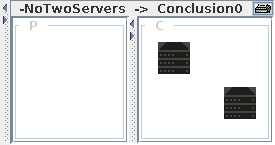
\includegraphics{grammar/no_two_servers}
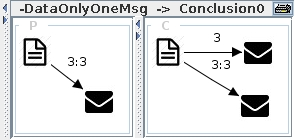
\includegraphics{grammar/data_no_two_msgs}
\caption{\label{fig:constraints} Negative atomic constraints for server}
\end{figure}

\subsection{Concurrent Rules Induced by Dependencies}

The default algorithm constructs the concurrent rules based on all the overlappings of the right side of the first rule and left side of the second rule, allowing us to see how the elements created/preserved by one rule can be connected with the elements deleted/preserved by the other.

One way to restrict the number of possible concurrent rules and still generate meaningful rules is to filter and use only the overlappings associated with dependencies~\cite{Lambers2006} between subsequent pairs of rules. The idea behind this is to use only the overlappings where (1) the elements needed for the second rule to be applied are explicitly created by the first one or (2) the elements forbidden by the NACs of the second rule are explicitly deleted by the first.

For the first case, we only need to filter the overlappings in the concurrent rule diagram where $\nexists h_{12} : R'_c \rightarrow C_n$ such that $(l_n \circ h_{12} = e_1$ and $r_n \circ h_{12} \models N^{-1}_i)$ or $\nexists h_{21} : L_n \rightarrow C_c$ such that $(r_c \circ h_{21} = e_2$ and $l_c \circ h_{21} \models N_j)$.

However, this notion does not take into consideration the elements whose existence is forbidden by the NACs of the second rule and would then forbid its application, but once deleted by the first rule the application of the second is enabled.

We did not find on the literature a construction to capture those cases, however an adaptation of the concurrent rule algorithm can be made based on the algorithm for calculating dependencies between the rules defined in~\cite{Lambers2006}. Besides the overlappings between $(R'_c, L_n)$ that represent dependencies, we generate \emph{also} the overlappings of the left side of the first rule $L'_c$ with the NACs $N_j$ and check whether the rewritings are possible, in which case the
diagram for the corresponding concurrent rule construction can be seen as follows:

\diagram{
    N_i& & & & N_j\ar@{.>}@/_3pc/[ddllll]_{e_2} & & \\
      L'_c\ar[u]^{n_i}\ar[d]_{e_1}\ar@{}[dr]|{(1)} & K'_c\ar[d]\ar[l]\ar[r] \ar@{}[dr]|{(2)} & R'_c\ar[dr]^{m'_1} & & L_n\ar[dl]_{m_2}\ar[u]^{n_j} & K_n\ar[d]\ar[l]\ar[r]\ar@{}[dl]|{(3)} & R_n\ar[d]^{m'_2}\ar@{}[dl]|{(4)}\\
        \textit{E} & C_c\ar[l]|{c_l}\ar[rr]|{c_r} & & P_1 & & C_n\ar[ll]|{n_l}\ar[r]|{n_r} & P_2\\
          & & & K\ar@{.>}@/1pc/[llu]|{k_c}\ar@{.>}@/1pc/[urr]|{k_n}\ar@{}[u]|{(5)} & & & 
          }\vspace{-15pt}


          \subsection{Maximal Concurrent Rule}

          Sometimes, instead of generating all possible overlappings or even all the dependencies, the modeller is interested in seeing only the maximal interactions between the elements of each rule in the sequence, thus we may filter the overlappings with the least number of elements, capturing the cases where the elements of each rule are as connected as possible. Note that the rule in Fig~\ref{fig:concurrent_rule_construction} is a maximal concurrent rule.


\section{Comparison or Results}

  \chapter{Verigraph Tool Overview}\label{ch:verigraph}

Verigraph~\cite{verigraph} is a new tool for simulating and analizing graph grammars implemented in Haskell\footnote{The source code is available at \url{https://github.com/Verites/verigraph}}, a purely functional programming language. The tool is being developed by the Verites group\footnote{\url{http://www.ufrgs.br/verites}} with two particular aims. The first one is to build a software tool that serves as an implementation of standard constructions and analysis for graph grammars, while also being as closely related to the theory as possible. The second, to provide a framework for exploring new ideas and techniques in graph grammars and other category theory related topics~\cite{BezerraETMF2016,Costa2016,CostaETMF2016, Becker2014}.

Regarding category theory, Verigraph implements important basic constructions such as coequalizers, coproducts, colimits, pushout complements, initial pushouts, pullbacks, negative application conditions, constraints, among others. The implementation of this constructions follows a very similar approach to the one used in~\cite{Rydeheard1988}, where categorial concepts are implemented as types in ML and constructive proofs of theorems in category theory are built as ML programs.

The implemented categorial constructions are used as a basis to implement several graph grammar analyses, such as critical pair analysis~\cite{Lambers2006}, state space generation and model checking~\cite{Becker2014}, concurrent rules generation~\cite{BezerraETMF2016} and higher-order graph transformations~\cite{Machado2015}. They were also used to implement the construction of occurrence graph grammars with NACs, which were explained in depth in chapter~\ref{ch:process}.

The analysis algorithms are implemented in a generic functional style, having the advantage of being very close to the formal definitions, thus making it easier to reason about them and to inspect for correctness. 
In addition, Verigraph benefits from a layered architecture, shown on Figure~\ref{fig:verigraph:layers}, where it is easy to reuse the same analysis algorithms (top layer) for other categories different than \cat{TGraph_T} (bottom layer), as long as they implement the contracts given
by the type classes (middle layer) defined on the system.
Examples of these type classes are shown on Figures~\ref{fig:verigraph:morphism-type-class} and \ref{fig:verigraph:cocomplete-type-class}.

\begin{figure}[!ht]
  \centering
  \begin{subfigure}[t]{.5\textwidth}
    \centerline{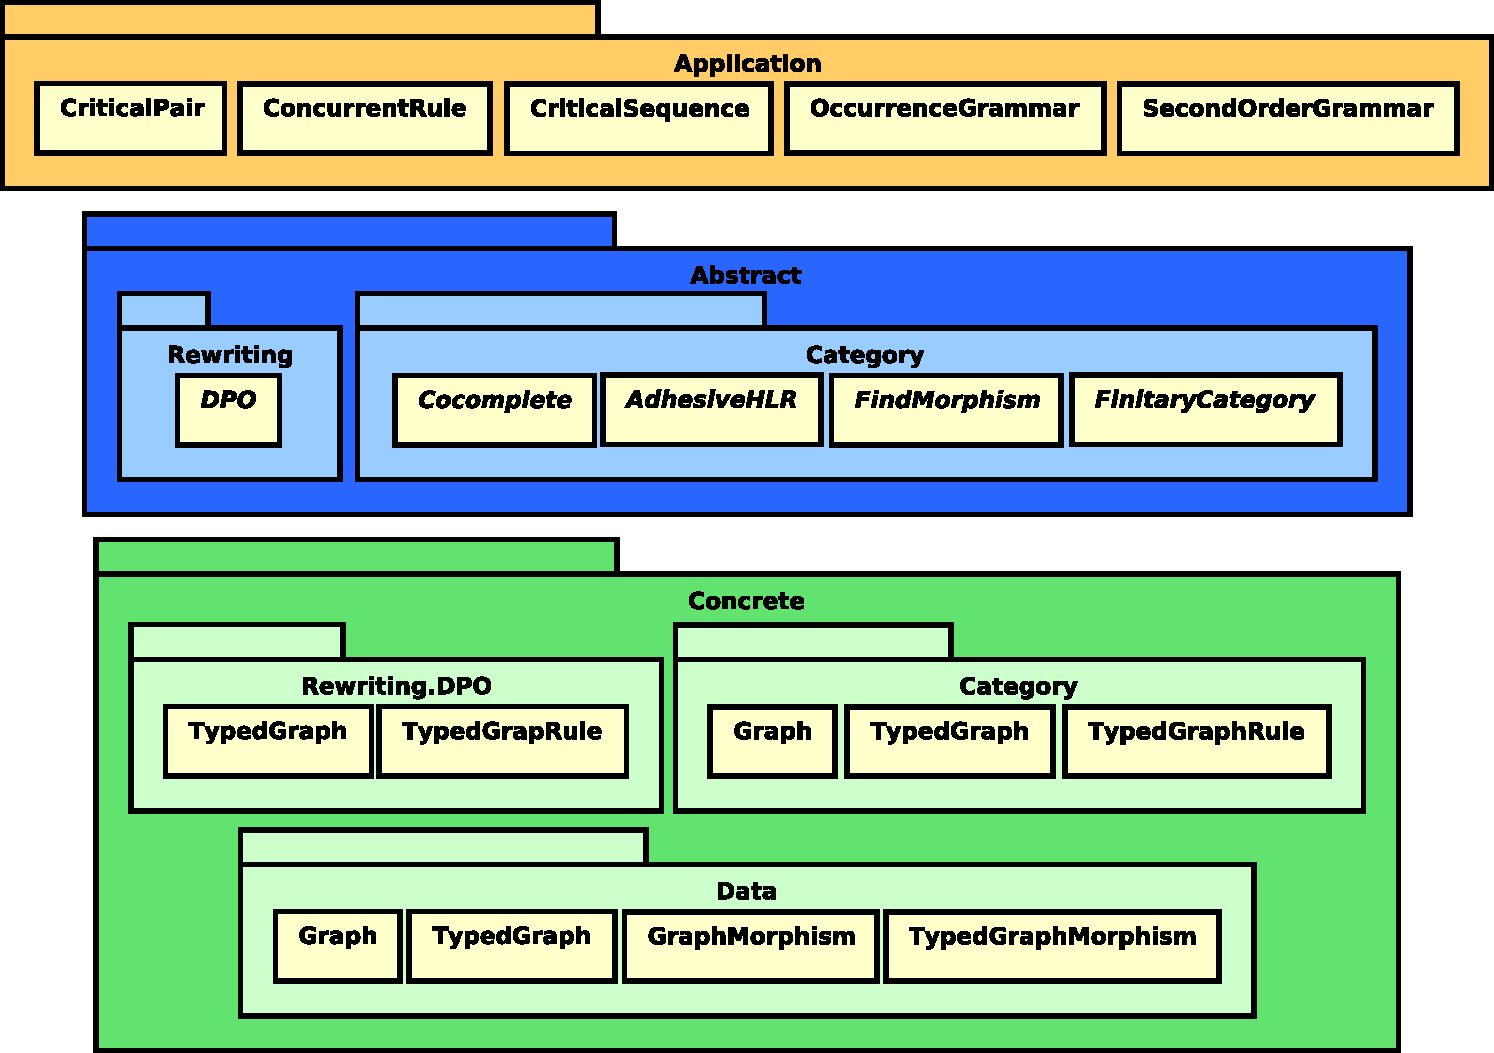
\includegraphics[scale=0.6]{images/verigraph/layers}}
%    \caption{Detailed Layers}
  \end{subfigure}
%  \begin{subfigure}[t]{.5\textwidth}
%    \centerline{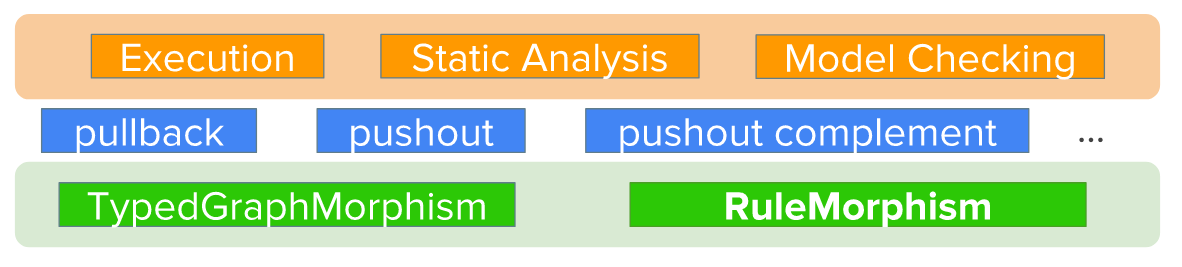
\includegraphics[scale=0.5]{images/verigraph/layers-abstract}}
%    \caption{Example}
%  \end{subfigure}%
  \caption{Verigraph architecture}\label{fig:verigraph:layers}
\end{figure}

There are tools for analysing graph grammars which are similar to Verigraph in some aspects, such as AGG~\cite{Taentzer2000} and GROOVE~\cite{Rensink2004}. Recently, \cite{Deckwerth2016} introduced a java framework for static verification of graph transformations also based in category theory.
  However, to our knowledge, Verigraph is the only tool that integrates static and dynamic analyses, second-order specifications and provides support for new categorial constructions and algorithms, besides being the only tool in this field implemented in a pure functional language~\cite{Costa2016}.
  Moreover, Verigraph is a free and open source software, available online for the community in one of the biggest platforms for software repositories currently available. In addition to it, not only its source code, but also its roadmap are public and open to suggestions and collaborations from outside the Verites group.

In the next sections of this chapter, we will demonstrate basic aspects of Verigraph implementation. First we present general categorial constructions which are the basic foundations of the tool; then we provide details about the implementation of concrete objects and categories, specifically focusing on \typedGraphCategory{}; after, we present the implementation of some analysis algorithms and show how they can be reused by other categories. %Finally, we explain in depth how the calculation of Occurrence Graph Grammars was implemented, which is part of our thesis contribution.

\section{Implementation of Categorial Constructions}

The first basic type class in Verigraph is \code{Morphism}, shown in Figure~\ref{fig:verigraph:morphism-type-class}, which serves as the minimal contract for any category to be implemented in the tool. Notice how the contract of this type class reflects the category definition (see Definition~\ref{def:category}).

\begin{figure}[!ht]
\caption{Morphism Type Class}
\begin{minted}[linenos=true, breaklines,fontsize=\small]{haskell}
class (Eq m) => Morphism m where
    type Obj m :: *
    compose  :: m -> m -> m
    domain   :: m -> Obj m
    codomain :: m -> Obj m
    id       :: Obj m -> m
    isMonomorphism :: m -> Bool
    isEpimorphism :: m -> Bool
    isIsomorphism :: m -> Bool
\end{minted}
\label{fig:verigraph:morphism-type-class}
\end{figure}

All the other type classes in the tool that are related to category theory are somehow defined in terms of \code{Morphism}. For example, the \code{Cocomplete} type class shown in Figure~\ref{fig:verigraph:cocomplete-type-class} defines some of the most basic categorial constructions used in Verigraph, such as coequalizers, coproducts and pushouts.

Notice that in the \code{Cocomplete} definition any category that implements the functions \code{calculateCoequalizer} and \code{calculateCoproduct} automatically will have a standard implementation of the \code{calculatePushout} function based only on these two constructions. This is due to the fact that, whenever a category has coequalizers and coproducts, it is possible to calculate any (finite) colimit based only on these two constructions, as demonstrated in~\cite{Pierce1991}.

We took advantage of this result to implement not only the \code{calculatePushout}, but also the calculation of the \code{colimit} of a diagram. The later being used in the generation of occurrence graph grammars as will be shown in chapter~\ref{ch:tests}.

Another interesting characteristic of the \code{Morphism} type class is that, even though \code{pushouts} and \code{colimits} are implemented in terms of \code{coproducts} and \code{coequalizers}, the programmer can override the default implementation and provide his/her own (categorial specific) implementation. This could be useful, for example, when for a given category \cat{C}, a particular algorithm to calculate the pushout is known to be more optimized than using the composition of basic operations.

\begin{figure}[!ht]
  \begin{minted}[linenos=true, breaklines, fontsize=\small]{haskell}
class (Morphism m) => Cocomplete m where
  calculateCoequalizer :: m -> m -> m
  calculateNCoequalizer :: NonEmpty m -> m
  calculateCoproduct :: Obj m -> Obj m -> (m,m)
  calculateNCoproduct :: NonEmpty (Obj m) -> [m]

  calculatePushout :: m -> m -> (m, m)
  calculatePushout f g = (f', g')
    where
      b = codomain f
      c = codomain g
      (b',c') = calculateCoproduct b c
      gc' = compose g c'
      fb' = compose f b'
      h = calculateCoequalizer fb' gc'
      g' = compose b' h
      f' = compose c' h
\end{minted}
\caption{Cocomplete Type Class}\label{fig:verigraph:cocomplete-type-class}
\end{figure}

In addition to \code{Morphism}, Verigraph has several other important type classes, some examples are:
\begin{itemize}
  \item \code{FindMorphism} for finding morphisms between objects of a category;
  \item \code{AdhesiveHLR} for operations that AdhesiveHLR categories (e.g. \cat{TGraph_T}) are guaranteed to have, such as calculating initial pushouts and pushout complements (when they exist);
  \item \code{DPO} for operations related to DPO graph rewriting approach, such as inversion of rules.
\end{itemize}

As for the concrete categories used, currently there are three specific implementations in Verigraph. Besides \cat{Graph} and \cat{TGraph_T}, which were reviewed on chapter~\ref{ch:gts}, there is also an implementation of \cat{TSpan_T}, where we have $T-$typed graph morphism spans are objects and span morphisms are arrows or, from a more concrete perspective, DPO graph rules as objects and morphisms between rules as arrows.

\section{Implementation of Graph Grammars}

The main concrete structures in Verigraph are (typed) graph grammars, which is currently the focus of the Verites group. The basic implementation begins with the \code{Graph} type, which consists of a list of nodes and a list of edges together with an API for graph manipulation with basic functions.

The \code{Graph} definition on Haskell is show on Figure~\ref{fig:verigraph:graph}. The \code{Graph} API is not shown, but it includes basic graph operations such as \code{insertNode}, \code{insertEdge}, \code{removeNode}, \code{removeEdge}, \code{incomingEdges}, \code{outgoinEdges}, \code{sourceOf}, \code{targetOf}, among others. 

\begin{figure}[!ht]

\caption{Graph implementation}
\begin{minted}[linenos=true, breaklines,fontsize=\small]{haskell}
data Node a = Node 
{ getNodePayload :: Maybe a
}

data Edge a = Edge 
{ getSource      :: NodeId
, getTarget      :: NodeId
, getEdgePayload :: Maybe a
}

data Graph a b = Graph 
{ nodeMap :: [(NodeId, Node a)]
, edgeMap :: [(EdgeId, Edge b)]
}
\end{minted}
\label{fig:verigraph:graph}
\end{figure}

We use \code{Graph} to progressively build the morphisms necessary to implement the categories \cat{Graph}, \cat{TGraph_T} and \cat{TSpan_T}. A graph morphism consists of a graph as domain, a graph as codomain and relations that map the nodes and edges in the domain graph to the ones in the codomain one. A typed graph is regarded as a simple graph morphism and a typed graph morphism consists of a typed graph as domain, a typed graph as codomain and a graph morphism relating the two of them.

Figure~\ref{fig:verigraph:concrete-morphisms} shows all categories currently implemented in Verigraph based on their morphisms. Moreover, all concrete morphisms presented implement the \code{Morphism} type class. Figure~\ref{fig:verigraph:morphism-implementation} shows how \code{TypedGraphMorphism} implements \code{Morphism} type class in order to provide the \cat{TGraph_T} category.

Similar implementations were done for \code{GraphMorphism} and \code{RuleMorphism}.

\begin{figure}[!ht]
\caption{Basic concrete morphisms of Verigraph.}
\begin{minted}[linenos=true, breaklines,fontsize=\small]{haskell}
data GraphMorphism a b = GraphMorphism 
{ getDomain    :: Graph a b
, getCodomain  :: Graph a b
, nodeRelation :: R.Relation G.NodeId
, edgeRelation :: R.Relation G.EdgeId
}

type TypedGraph a b = GraphMorphism a b

data TypedGraphMorphism a b = TypedGraphMorphism 
{ getDomain   :: TypedGraph a b
, getCodomain :: TypedGraph a b
, mapping     :: GraphMorphism a b
}

data RuleMorphism a b = RuleMorphism 
{ rmDomain         :: Production (TypedGraphMorphism a b)
, rmCodomain       :: Production (TypedGraphMorphism a b)
, mappingLeft      :: TypedGraphMorphism a b
, mappingInterface :: TypedGraphMorphism a b
, mappingRight     :: TypedGraphMorphism a b
}
\end{minted}
\label{fig:verigraph:concrete-morphisms}
\end{figure}

\begin{figure}[!ht]
\caption{Typed graph morphism implementing morphism type class.}
\begin{minted}[linenos=true, breaklines,fontsize=\small]{haskell}
instance Morphism (TypedGraphMorphism a b) where
  type Obj (TypedGraphMorphism a b) = TypedGraph a b
  domain = getDomain
  codomain = getCodomain
  compose t1 t2 = TypedGraphMorphism (domain t1) (codomain t2) $ compose (mapping t1) (mapping t2)
  id t = TypedGraphMorphism t t (M.id $ domain t)
  isMonomorphism = isMonomorphism . mapping
  isEpimorphism = isEpimorphism . mapping
  isIsomorphism = isIsomorphism . mapping
\end{minted}
\label{fig:verigraph:morphism-implementation}
\end{figure}

\section{Implementation of the Analysis Algorithms}

The analysis algorithms are also implemented at a high level of abstraction, based on categorial definitions and their implementation as type classes. For example, the code for calculating conflicts or dependencies between two rules was first implemented for \cat{TGraph_T}, but since it is based on the abstraction of \code{DPO} type class this piece of code can be reused by any other category implementing the \code{DPO} contract.

Furthermore, Figure~\ref{fig:verigraph:delete-use-produce-use} shows a piece of code with functions responsible to test whether an overlapping pair of two rules rises a conflict or a dependency for one of those rules. Notice how this code resembles the definitions of delete-use conflict (Definition~\ref{def:classic-conflict}) and produce-use dependency (Definition~\ref{def:classic-dependency}).


\begin{figure}[!ht]
\caption{Delete-Use and Produce-Use Implementation}
\begin{minted}[linenos=true, breaklines,fontsize=\small]{haskell}
-- | Rule @p1@ is in a delete-use conflict with @p2@ if @p1@ deletes something that is used by @p2@. This function verifies the non existence of h21: L2 -> D1 such that d1 . h21 = m2
isDeleteUse :: (DPO m) => Production m -> (m, m) -> Bool
isDeleteUse p1 (m1,m2) = null h21
  where
    --gets only the morphism d1 from D1 to G
    (_,d1) = calculatePushoutComplement m1 (getLHS p1) 
    h21 = findAllPossibleH21 m2 d1

isProduceUse :: (DPO m) => Production m -> (m, m) -> Bool
isProduceUse p1 (m1',m2) = null h21
  where
   --gets only the morphism d1 from D1 to G
   (_,e1) = calculatePushoutComplement m1' (getRHS p1)
   h21 = findAllPossibleH21 m2 e1
\end{minted}
\label{fig:verigraph:delete-use-produce-use}
\end{figure}

As an example of its application at other categories we have \cat{TSpan_T}, which also implements the \code{DPO} type class and benefits from the same algorithms for finding conflicts and dependencies. This also can be used for different categories based on graphs, algebras, logics and so on.

Besides basic categorial constructions and several analysis techniques for graph grammars, Verigraph was also used to implement the construction of Occurrence Graph Grammars and the relations presented in chapter~\ref{ch:process}. This construction is presented in more detail in the following chapter.



  \chapter{Methodology}

\section{Presentation of the original methodology}

\section{Extensions to deal with interactions among Use Cases and other documents}

\section{Other improvements}

\section{Patterns}
Appendix?

\cite{Junior2015}


  \chapter{Case Study}

\iffalse 
$L1$ is a simple call-by-value functional language with high order functions. All functions are currified, that is, have exactly one argument.

\begin{figure}
  \caption{$L1$ Abstract Syntax}
  \begin{openframe}
    \begin{align*}
      e ::= & \quad n \quad |\quad x \quad | \quad e_1 \: op \: e_2 \\
        & |\quad \text{if } e_1 \text{ then } e_2 \text{ else } e_3 \\
        & |\quad e_1 e_2 \\
        & |\quad \text{fn x } \Rightarrow e \\
        & |\quad \text{let y } = e_1 \text{ in } e_2 \\
        & |\quad \text{letrec y } = (\text{fn x } \Rightarrow e_1) \text{ in } e_2 \\
    \end{align*}

    where

    \begin{align*}
      n & \in \mathbb{N} \\
      x & \in \text{set of variable identifiers} \\
      op & \in \{+, -, *, /,  =, <, >, \geq, \leq \} \\
    \end{align*}
  \end{openframe}
\end{figure}

Acqua goal is to explore parallel execution of function applications. A classical example that allows to explore parallel function applications is the algorithm to find the n-th number of the Fibonacci sequence. The Fibonacci number sequece starts with the number 1 two times, and all other numbers are the result of the sum of the last two numbers. Thus, the sequence is \{1,1,2,3,5,8,13,...\}.

The figure \ref{fig:fib-l1} shows a naive $L1$ program that finds the 7th number on the Fibonacci sequence. The recursive function fibo is declared on the first line. The second line shows that fibo is a function that receives one argument (as any function on $L1$) named $x$. The lines 3-5 are the body of the function, that returns 1 when $x$ is less than 2, or the sum of two fibo applications, for $x-1$ and $x-2$. The lines 6 and 8 limit the scope of this function definition. On the line 7 we have the application of the function fibo to the number 7, thus, finding the 7th number of the Fibonacci sequence.

\begin{figure}
  \caption{Fibonacci function applied to 7}
  \begin{lstlisting}[language=l1]
letrec fibo =
  fn x =>
    if x < 2
      then 1
      else (fibo (x - 1)) + (fibo (x - 2))
in
  fibo 7
end
  \end{lstlisting}
  \label{fig:fib-l1}
\end{figure}

To find the 7th Fibonacci number, we need to first find the 6th and 5th numbers. And for the 6th, we need the 5th and 4th numbers. We can represent this dependency using a tree, as show in figure \ref{fig:fibo}. This tree will have the height of $n-2$, except when we are calculating the first and second numbers of fibonacci sequence. This is so because for any node, the subtree on the right is contained on the subtree on the left. So to find the height we only need to consider the leftmost path. The width of this tree is the own fibonacci number. This is so because the width of the first and second numbers are 1, and the width of $n$ is the width of $(n-1) + (n-2)$.

\begin{figure}
    \caption{Fibonacci sequence tree}
    \centerline{
      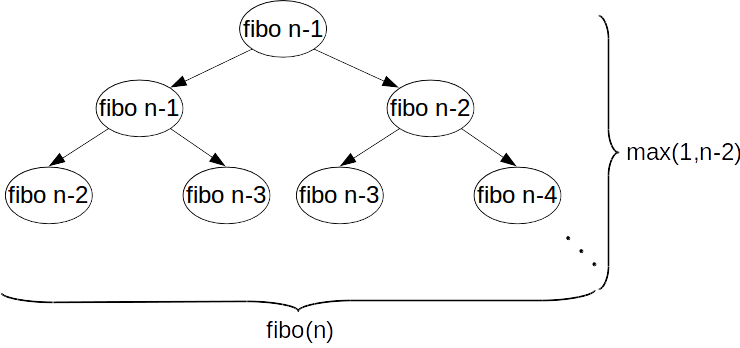
\includegraphics[width=0.7\textwidth]{fibo.png}
    }
    \label{fig:fibo}
\end{figure}

Each node in the Fibonacci dependency tree represents a function application in the program shown on figure \ref{fig:fib-l1}. The acqua architecture allows function applications to be done in parallel, so the architecture has the potential to parallelize the width of the tree in a given moment, that is $fibo(n)$ function applications. Function application will generate a job, and each job will potentially copy one environment with only two name bindings: The $x$ variable and the reference to $fibo$ function, thus the environment copy is constant. Assuming that we have enough processing units in the architecture, we can execute the naive program shown on figure \ref{fig:fib-l1} in linear time.
\fi

  \chapter{Related Work}\label{ch:related-work}

There exists a wide range of model-based techniques to test generation~\cite{Utting2006}, however due to the scope of our work we will focus on those based on graph transformation systems.

The advantages of graph transformation systems over other models are...

\section{Unfolding}

Code generators are a set of tools used to translate graphical specifications of systems directly into executable code. According to \cite{Baldan2004}, they are widely used in the development of embedded software, e.g. in the automotive sector, however they lack the maturity and testing when compared to compilers of standard programming languages.

According to them, one of the biggest problems is testing code generators is the difficulty to describe the transformation rules from the graphical model to the target language as well as the interactions amongst them in a precise and formal way. Therefore, the authors propose a graph transformation based approach for systematically deriving test cases in this particular scenario.

Their approach is based on the use of unfolding of graph transformation systems~\cite{Ribeiro1996} over two graph grammars, a \textit{generating grammar}, responsible for generating all possible input models, and an \textit{optimising grammar}, which formalises specific transformation steps towards code optimization.

The purpose

The results

The limitations: nacs extend the match with only one edge and are weaker than general nacs, isolated nodes are irrelevant, 

acyclic graphs and maximal depth of the unfolding

\section{Visual Contracts}

An approach proposed by~\cite{Heckel2011},~\cite{Khan2012},~\cite{Khan2012a},~\cite{Runge2013} focusing mainly on generating test cases for service-oriented or component-based systems. Given that systems of this kind often hide their implementation, the authors use interface descriptions known as visual contracts\footnote{ Formally regarded as graph transformation rules with operation signatures}, in order to model the observable behaviour of the system.

Coverage criteria is defined by means of static analysis, where potential conflicts and dependencies amongst visual contracts are calculated and used to build a dependency graph. In this situation, despite of being called ``a dependency graph'', this structure is rather similar to our occurrence relation, summarizing the results of both conflict and dependency analysis while representing the possible orderings in which the visual contracts may be executed.

In the processes of generating test cases, it is necessary to provide also an initial graph, which is used to find out which visual contracts are applicable to it. One of such visual contracts is chosen as the first step and all the paths through the dependency graph in which each rule is applied at most once are computed and stored as a set of rule sequences. Thereafter, the sequences are enriched to encompass rules with multiple dependencies and lately redundant rules contained in larger ones are
removed. Afterwards, each sequence is executed (if possible), and any new edges in the dependency graph reached by them are added to coverage. The entire process is then repeated as long as the coverage shows improvements. 

In comparison to our work, this approach has both advantages and limitations. As an example of the first, there are: the possibility to work with attributed typed graph transformation systems and multi-rules. As for the second: it requires more user involvement during the process of test case generation, it does not enclose negative application conditions, it was planned to work in a configuration where each rule is applied at most once and although being an extension of
AGG~\cite{Taentzer2000}, the tool is not available to download.

\section{Other Tools}

Overview and Comparison with other tools

\begin{itemize}
\item AGG
\item Groove
\item Henshin
\item AutoGraph
\item Deckwerth Framework
\end{itemize}

\section{Other methods for model-based test generation}

\begin{itemize}
  \item Finite State Machines
  \item UML
  \item Pre/Post Models
\end{itemize}


  \chapter{Conclusions}

\section{Future Work}

\begin{itemize}
  \item Investigate Conflicts, Dependencies and Local Church-Rosser with Graph Constraints
  \item NACs over concrete elements of the core graph and not only over the type graph. 
  \item Compile general NACs to incremental NACs
  \item Investigate whether there are a better algorithm than backtracking to compute occurrence relations
  \item GUI for presenting Doubly-Typed Graph Grammars
\end{itemize}


%% aqui comeca o texto propriamente dito
%
%\section{Figuras e tabelas}
%
%Esta seção faz referência às Figuras~\ref{fig:estrutura},~\ref{fig:ex1} e~\ref{fig:ex2}, a título de exemplo. A primeira figura apresenta a estrutura de uma figura. A \emph{descrição} deve aparecer \textbf{acima} da figura. Abaixo da figura, deve ser indicado a origem da imagem, mesmo se essa for apenas os autores do texto.
%
%A Figura~\ref{fig:ex1} representa o caso mais comum, onde a figura propriamente dita é importada de um arquivo (neste exemplo em formato \texttt{eps} ou \texttt{pdf}. Veja a seção \ref{sec:fig_format}). A Figura~\ref{fig:ex2} exemplifica o uso do environment \texttt{picture}, para desenhar usando o próprio~\LaTeX.
%
%\begin{figure}[h]
%    \caption{Descrição da Figura deve ir no topo}
%    \begin{center}
%        % Aqui vai um includegraphics , um picture environment ou qualquer
%        % outro comando necessário para incorporar o formato de imagem
%        % utilizado.
%        \begin{picture}(100,100)
%                \put(0,0){\line(0,1){100}}
%                \put(0,0){\line(1,0){100}}
%                \put(100,100){\line(0,-1){100}}
%                \put(100,100){\line(-1,0){100}}
%                \put(10,50){Uma Imagem}
%        \end{picture}
%    \end{center}
%    \label{fig:estrutura}
%    \legend{Fonte: Os Autores}
%\end{figure}
%
%\begin{figure}
%    \caption{Exemplo de figura importada de um arquivo e também exemplo de caption muito grande que ocupa mais de uma linha na Lista~de~Figuras}
%    \centerline{\includegraphics[width=8em]{fig}}
%    \legend{Fonte: Os Autores}
%    \label{fig:ex1}
%\end{figure}
%
%% o `[h]' abaixo é um parâmetro opcional que sugere que o LaTeX coloque a
%% figura exatamente neste ponto do texto. Somente preocupe-se com esse tipo
%% de formatação quando o texto estiver completamente pronto (uma frase a mais
%% pode fazer o LaTeX mudar completamente de idéia sobre onde colocar as
%% figuras e tabelas)
%%\begin{figure}[h]
%\begin{figure}
%    \caption{Exemplo de figura desenhada com o environment \texttt{picture}.}
%    \begin{center}
%        \setlength{\unitlength}{.1em}
%        \begin{picture}(100,100)
%                \put(20,20){\circle{20}}
%                \put(20,20){\small\makebox(0,0){a}}
%                \put(80,80){\circle{20}}
%                \put(80,80){\small\makebox(0,0){b}}
%                \put(28,28){\vector(1,1){44}}
%        \end{picture}
%    \end{center}
%    \legend{Fonte: Os Autores}
%    \label{fig:ex2}
%\end{figure}
%
%Tabelas são construídas com praticamente os mesmos comandos. Ver a tabela \ref{tbl:ex1}.
%
%\begin{table}[h]
%    \caption{Uma tabela de Exemplo}
%    \begin{center}
%        \begin{tabular}{c|c|p{5cm}}
%            \textit{Col 1}  &   \textit{Col 2}  &   \textit{Col 3} \\
%            \hline
%            \hline
%            Val 1           &   Val 2           & Esta coluna funciona como um parágrafo, tendo uma margem definida em 5cm. Quebras de linha funcionam como em qualquer parágrafo do tex. \\
%            Valor Longo     & Val 2             & Val 3 \\
%            \hline
%        \end{tabular}
%    \end{center}
%    \legend{Fonte: Os Autores}
%    \label{tbl:ex1}
%\end{table}
%
%\subsection{Formato de Figuras}
%\label{sec:fig_format}
%
%O LaTeX permite utilizar vários formatos de figuras, entre eles \emph{eps}, \emph{pdf}, \emph{jpeg} e \emph{png}. Programas de diagramação como Inkscape (e mesmo LibreOffice) permitem gerar arquivos de imagens vetoriais que podem ser utilizados pelo LaTeX sem dificuldade. Pacotes externos permitem utilizar SVG e outros formatos.
%
%Dia e xfig são programas utilizados por dinossauros para gerar figuras vetoriais. Se possível, evite-os.
%
%\subsection{Classificação dos etc.}
%
%O formato adotado pela ABNT prevê apenas três níveis (capítulo, seção e subseção). Assim, \texttt{\char'134subsubsection} não é aconselhado.
%
%\section{Sobre as referências bibliográficas}
%
%A classe \emph{iiufrgs} faz uso do pacote \emph{abnTeX2} com algumas alterações
%feitas por Sandro Rama Fiorini. Culpe ele se algo der errado. Agradeça a ele
%pelo que der certo. As modificações dão uma camada de tinta NATBIB-style,
%já que o abntex2 usa uns comandos de citação feitos para alienígenas de 5 braços 
%wtf. Exemplos de citação:
%
%\begin{itemize}
%    \item \emph{cite}: Unicórnios são verdes \cite{Adams2009Conceptual};
%    \item \emph{citep}:Unicórnios são verdes \citep{Adams2009Conceptual};
%    \item \emph{citet}: Segundo \citet{Adams2009Conceptual}, unicórnios são
%                        verdes.
%    \item \emph{citen or citenum}: Segundo \citen{Adams2009Conceptual},
%        unicórnios são verdes.
%    \item \emph{citeauthor e citeyearpar}: Segundo artigos de
%        \citeauthor{Adams2009Conceptual} , unicórnios são verdes 
%        \citeyearpar{Adams2009Conceptual}.
%
%\end{itemize}
%
%O estilo abnt fornecido antigamente pelo UTUG não é mais recomendado, pois não
%produz saída de acordo com as exigências da biblioteca.
%
%Recomenda-se o uso de bibtex para gerenciar as referências (veja o arquivo
%biblio.bib).
%
%% e aqui vai a parte principal
%%
%% \chapter{Estado da arte}
%% \chapter{Mais estado da arte}
%% \chapter{A minha contribuição}
%% \chapter{Prova de que a minha contribuição é válida}
%% \chapter{Conclusão}
%
%% referencias
%% aqui será usado o environment padrao `thebibliography'; porém, sugere-se
%% seriamente o uso de BibTeX e do estilo abnt.bst (veja na página do
%% UTUG)
%%
%% observe também o estilo meio estranho de alguns labels; isso é
%% devido ao uso do pacote `natbib', que permite fazer citações de
%% autores, ano, e diversas combinações desses
%
\bibliographystyle{abntex2-alf}
\bibliography{biblio}
\end{document}
